\documentclass[11pt,a4paper]{article}

% \usepackage{times}

% \usepackage{enumitem}

\usepackage{textcomp}

\usepackage{gensymb}

\usepackage{array}

\usepackage{amsmath}

\usepackage{amssymb}

\usepackage{amsfonts}

\usepackage[notes,backend=biber,useibid=true]{biblatex-chicago}
\bibliography{bib}

% \bibliography{bailey}

\usepackage{pgfplots}

\pgfplotsset{width=10cm,compat=1.9}

\usepgfplotslibrary{external}



\tikzexternalize



\usepackage{multirow}



\usepackage[utf8]{inputenc} % set input encoding (not needed with XeLaTeX)

%\usepackage[defaultfam,tabular,lining]{montserrat} %% Option 'defaultfam'

%% only if the base font of the document is to be sans serif

%\usepackage[T1]{fontenc}

%\renewcommand*\oldstylenums[1]{{\fontfamily{Montserrat-TOsF}\selectfont #1}}



%%% Examples of Article customizations

% These packages are optional, depending whether you want the features they provide.

% See the LaTeX Companion or other references for full information.



%%% PAGE DIMENSIONS

\usepackage[a4paper,margin=1in]{geometry}

% \usepackage{geometry} % to change the page dimensions

% \geometry{a4paper} % or letterpaper (US) or a5paper or....

% \geometry{margin=1in} % for example, change the margins to 2 inches all round

% \geometry{landscape} % set up the page for landscape

%   read geometry.pdf for detailed page layout information



\usepackage{graphicx} % support the \includegraphics command and options



% \usepackage[parfill]{parskip} % Activate to begin paragraphs with an empty line rather than an indent



%%% PACKAGES

\usepackage{booktabs} % for much better looking tables

\usepackage{array} % for better arrays (eg matrices) in maths

\usepackage{paralist} % very flexible & customisable lists (eg. enumerate/itemize, etc.)

\usepackage{verbatim} % adds environment for commenting out blocks of text & for better verbatim

\usepackage{subfig} % make it possible to include more than one captioned figure/table in a single float

% These packages are all incorporated in the memoir class to one degree or another...



%%% HEADERS & FOOTERS

\usepackage{fancyhdr} % This should be set AFTER setting up the page geometry

\pagestyle{fancy} % options: empty , plain , fancy

\renewcommand{\headrulewidth}{0pt} % customise the layout...

\lhead{}\chead{}\rhead{}

\lfoot{}\cfoot{\thepage}\rfoot{}



%%% SECTION TITLE APPEARANCE

\usepackage{sectsty}

% \allsectionsfont{\sffamily\mdseries\upshape} % (See the fntguide.pdf for font help)

% (This matches ConTeXt defaults)

% \renewcommand{\familydefault}{\sfdefault}





%%% ToC (table of contents) APPEARANCE

\usepackage[nottoc,notlof,notlot]{tocbibind} % Put the bibliography in the ToC

\usepackage[titles,subfigure]{tocloft} % Alter the style of the Table of Contents

\renewcommand{\cftsecfont}{\rmfamily\mdseries\upshape}

\renewcommand{\cftsecpagefont}{\rmfamily\mdseries\upshape} % No bold!



%%% END Article customizations



%%% The "real" document content comes below...





%%% Figure Template

% \begin{figure}[h!]

%	 \centering

%	 \includegraphics[height=6cm]{pendulum1}

%	 \caption{Diagram of a simple pendulum}

% \end{figure}

%%%



\usepackage{verbatim}



%%% Tikz Figure Template

\begin{comment}

\begin{figure}[h!]

	\begin{center}

		\begin{tikzpicture}

		\begin{axis}[

		title={},

		xlabel={Mass (kg)},

		ylabel={Period (s)},

		xmin=0, xmax=0.5,

		ymin=0, ymax=4,

		xtick={0,0.1,0.2,0.3,0.4,0.5},

		ytick={1,2,3,4},

		legend pos=north west,

		ymajorgrids=true,

		grid style=dashed,

		]

		

		\addplot[

		color=black,

		mark=o,

		]

		coordinates {

			(0.448,2.065)(0.289,2.063)(0.154,2.075)(0.098,2.067)

		};

		

		\end{axis}

		\end{tikzpicture}

		\caption{Relationship between period and mass}

	\end{center}

\end{figure}

\end{comment}





\title{Classification of Myers-Briggs Type Indicator (MBTI) Type Based on Past Posts on Internet Forums}

\author{Vincent Leonardo\\Selvam Shwetha\\Sun Kairan}

% \date{} % Activate to display a given date or no date (if empty),

% otherwise the current date is printed 





\begin{document}
	
	\maketitle
	
	\vfill
	\begin{center}
			GitHub repository link: \texttt{https://github.com/placid-brain/CDS-Project-2021}
	\end{center}

	\newpage
	
	\tableofcontents
	\newpage

	\section{Introduction}
	
	The rise of the Myers-Briggs Type Indicator (MBTI) as one of the most popular personality test in the past decade as part of the greater mainstream usage of personality types in popular culture is not surprising, at the very least. It functions as a framework in understanding one’s psychological tendencies through profiling four different dichotomies: Extraversion/Introversion (E/I), Sensing/Intuition (S/N), Thinking/Feeling (T/F), and Judging/Perceiving (J/P).\autocite{myersGiftsDifferingUnderstanding1995} Part of its widespread appeal can be attributed to the ease of use and interpretation of the model.\autocite{choongPredictingJudgingperceivingMyersBriggs2021} Self-assessments—oftentimes through the internet—allow for a democratisation of the personality test.\autocite{choongPredictingJudgingperceivingMyersBriggs2021} The four-letter MBTI types are also then interpretable through tangible and understandable names (e.g. “The Architect”, “The Mediator”, etc.) as an extension thereof (Keirsey Temperament Sorter) and descriptions that highlight the personalities’ assumed best traits.\autocite{lilienfeldSciencePseudoscienceClinical2014}
	
	Within more established organisations, there is also a desire for a personality framework that can be easily used in order to optimise working relationships and to create more efficient groupings of people of varying types.\autocite{lakeTrustNameBrand2019} In this case, there is more emphasis on justifying the use of the MBTI in these places. Oft-cited justifications include the Jungian basis as mentioned by its founders, Katherince Briggs and Isabel Myers. While Carl Jung’s contributions to the domain of psychology and psychoanalysis cannot be disputed, the nature of his work on psychological types cannot be considered scientifically rigorous.\autocite{carrollMyersBriggsTypeIndicator} As such, the Jungian basis cannot be used as a justification for the scientific nature of the MBTI, neither can the various studies endorsing it (many studies are either written by beneficiaries of the sales of the MBTI, methodologically weak, or both).\autocite{coffieldLearningStylesPedagogy2004}
	
	As a part of the popular internet culture, observations of social media biographies indicate that the MBTI has become a way to communicate one’s identity and preferences along with other indicators, heralding from astrology (e.g. Pisces, Virgo, etc.) or even fiction (e.g. Hogwarts’ Slytherin House from Harry Potter). The appearances of the MBTI alongside these indicators form the basis of one of the main criticisms on the personality test. A phenomenon described as the Barnum effect (or the Forer effect) can be used as a framework in describing the MBTI’s rise in popularity.\autocite{tobacykParanormalBeliefsBarnum1988} In this case, the descriptors of the personality can be said to be vague enough to be applicable to almost everyone, while being somewhat specific enough to allow for the feeling that it was specifically tailored for the particular person.
	
	While there are various criticisms on the usage of the MBTI, it is possible to observe that the widespread and democratising effect of the usage of the MBTI may lead to more scientifically rigorous methods. One such personality type construct is the Big Five Inventory, of which some correlations between its factors and MBTI dichotomies were found.\autocite{costajrRevisedNeoPersonality2008} Although its creation and the studies on it that follow may have scientific gaps, the inference of the MBTI type seemed to have been influential in the field of social media advertisement personalisation.\autocite{yiMBTIBasedCollaborativeRecommendation2016} The use of this technique has proven to positively impact consumer brand engagement, brand attachment, and subsequently revenue.\autocite{yoonEffectBigFive2018}
	
	Within this context, therefore, the usage of open social media posts by various users can be used to either predict the users’ MBTI types or to validate their self-reported assessments and types. The current research on the matter have had successes in predicting the four binary dichotomies separately.\autocite{yamadaIncorporatingTextualInformation2019} However, the predictive power of the MBTI type will be penalised quite severely due to the nature of having four independent probabilities combined together. Knowing that all four dichotomies are predictable at around 90\% accuracy each in various researches, it averages out to around 66\% accuracy when combined together.\autocite{choongPredictingJudgingperceivingMyersBriggs2021} This is significant as even a single letter difference in the prediction makes a noticeable difference in the types of recommendations and assumptions of the person assessed.\autocite{choongPredictingJudgingperceivingMyersBriggs2021}
	
	As such, the focus of this research will be on the holistic prediction of MBTI based on textual contents written by users of a social media platform. The methods of processing the textual data will be discussed, both in terms of its shape and transformations. Afterwards, a discussion on the model best suited for this classification task will be shown, followed by the choice for good baseline models. In the end, there will be an exploration on the models chosen in the attempt to improve on them or to combine them.
	
	\newpage
	\section{Dataset}
	
	\subsection{Source}

	The dataset being used will be from Kaggle, named `(MBTI) Myers-Briggs Personality Type Dataset'.\autocite{MBTIMyersBriggsPersonality} It contains two columns: a section of the last fifty posts by each user, separated by three pipe characters (“\textbar\textbar\textbar”) and the users' MBTI type. Each row is represented by a user from the PersonalityCafe forum, a social media site mainly focused on discussions on the self and personality types. In total, there are about 8600 rows of data.
	
	\subsection{Exploratory analysis}
	
	\begin{figure}[h!]
		\centering
		
		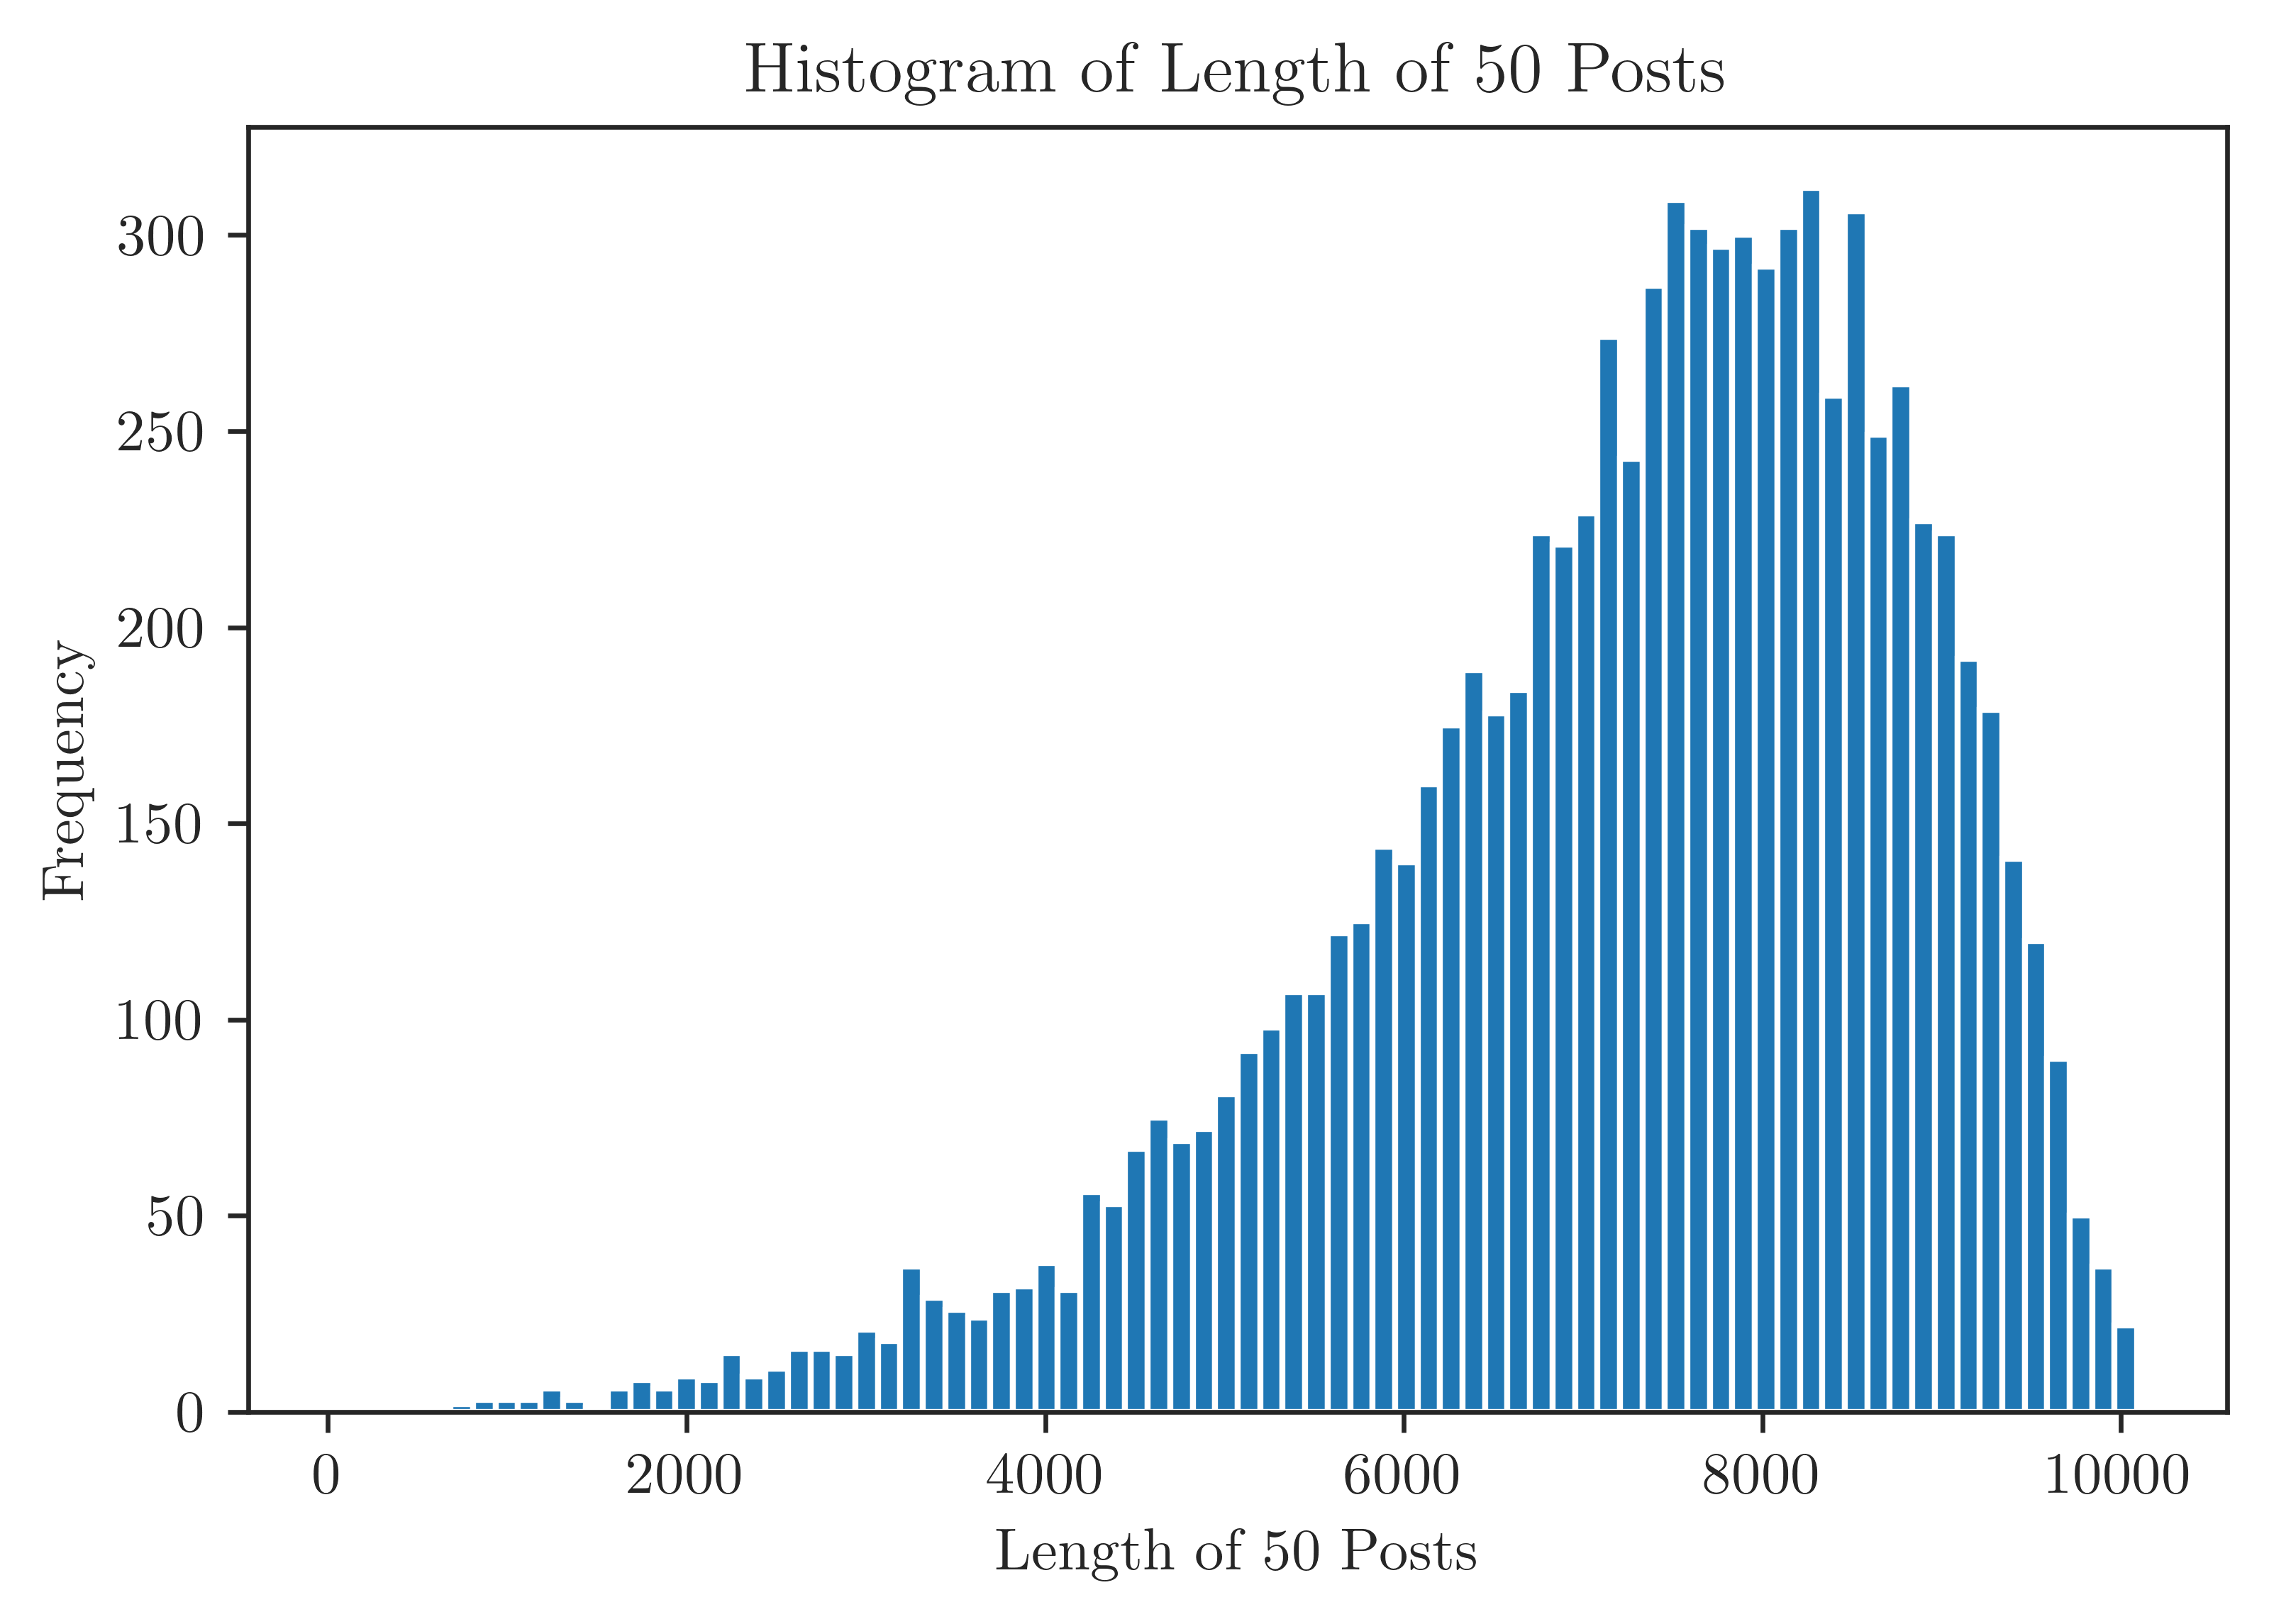
\includegraphics[height=8cm]{../output/visualisations/histogram_len_post}
		
		\caption{Histogram of the length of posts in the dataset}
		
	\end{figure}
	
	The lengths of the posts seem to be negatively skewed with a somewhat positive kurtosis. This indicates a consistency for the aggregate of fifty posts to be further from zero, which is advantageous as there are, in general, more data to work with per user. When considering the average length of posts when divided into the different types, there does not seem to be any appreciable difference in the distributions as seen in Figure 2.
	
%	\begin{table}[h!]
%		\centering
%		\begin{tabular}{ll}
%			\textbf{Descriptive statistics} & \textbf{Value} \\ \hline
%			Mean               & 7234.989625 \\
%		Standard deviation & 1607.806938 \\
%		Minimum            & 57          \\
%			First quartile     & 6325        \\
%			Median             & 7515        \\
%		Third quartile     & 8429        \\
%			Maximum            & 10090      
%		\end{tabular}
%	\caption{Descriptive analytics for the lengths of posts}
%	\end{table}

	\begin{figure}[h!]
		\centering
		
		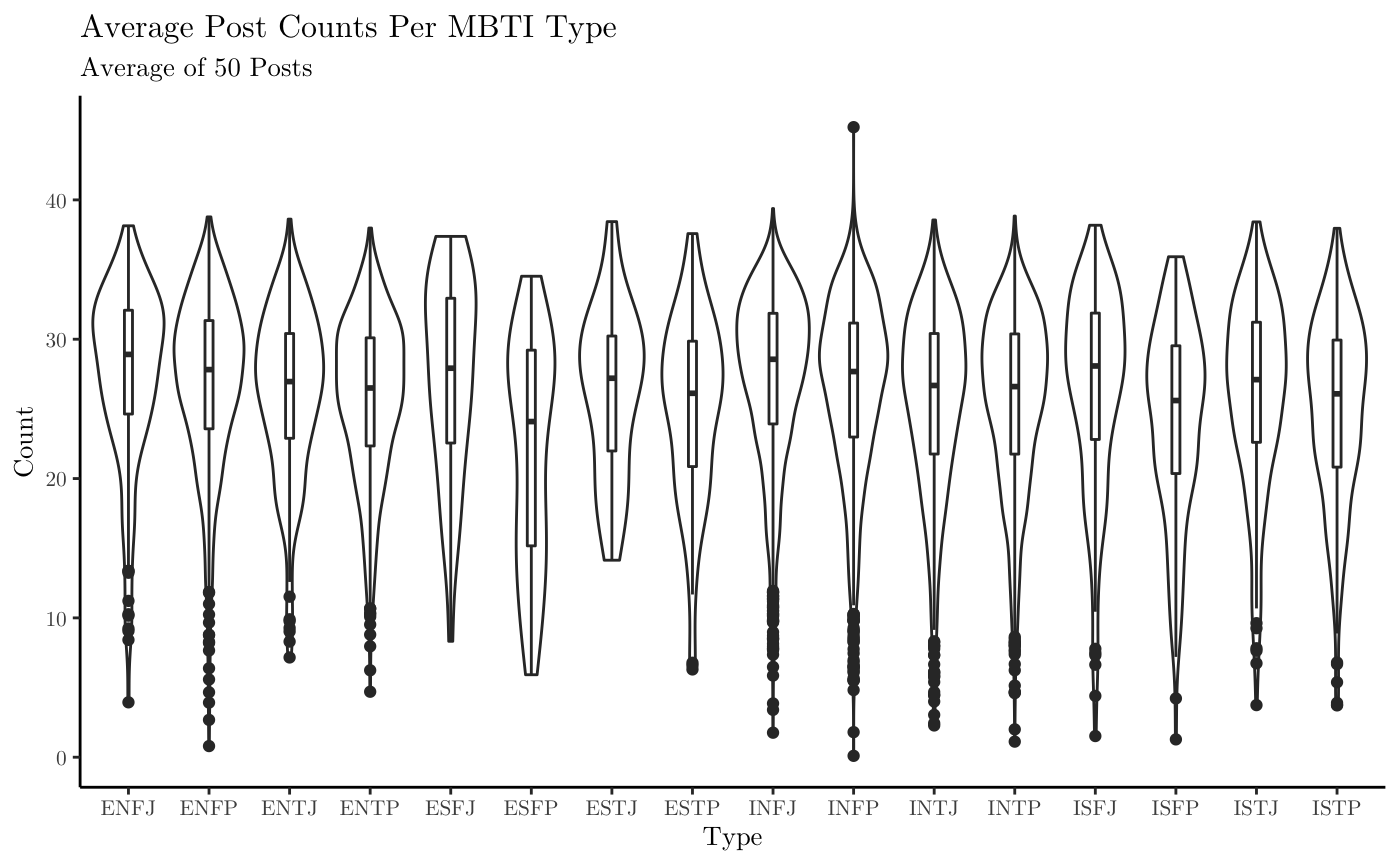
\includegraphics[height=8.5cm]{../output/visualisations/len_post_type}
		
		\caption{Average length of posts within each type}
		
	\end{figure}
	
	\begin{figure}[h!]
		\centering
		
		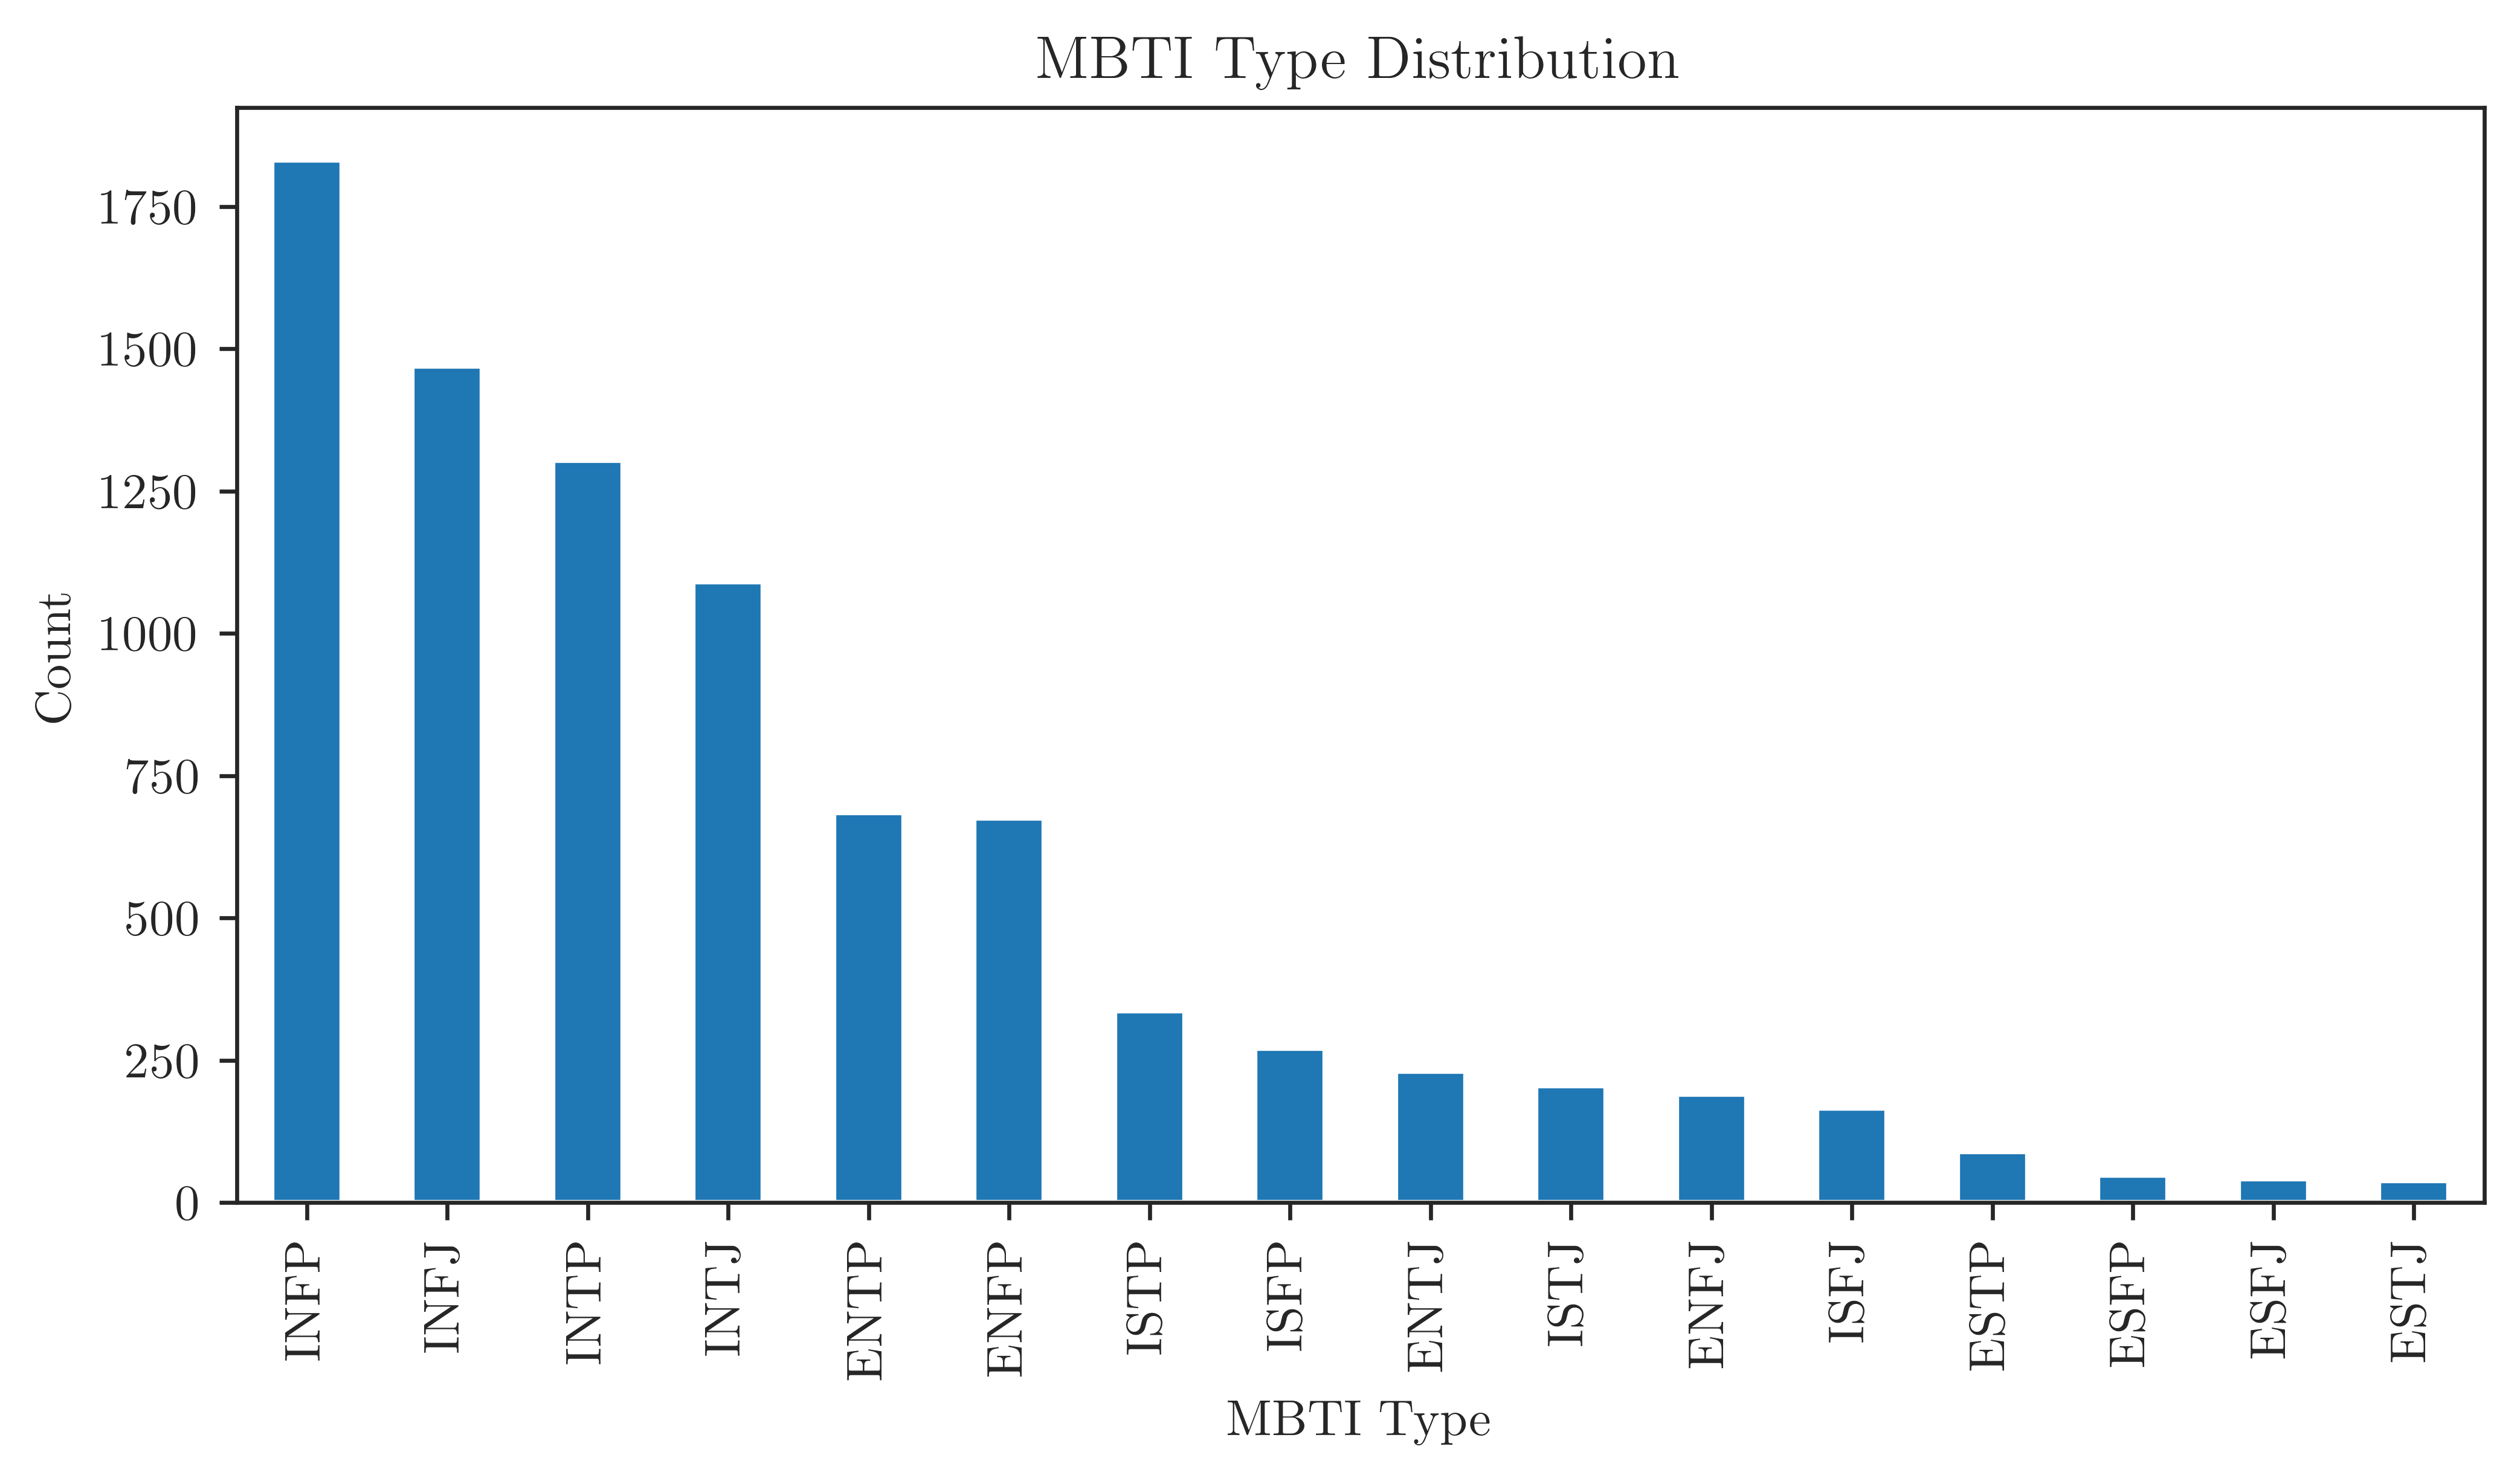
\includegraphics[height=8cm]{../output/visualisations/class_dist}
		
		\caption{Population distribution of the MBTI types}
		
	\end{figure}



	However, the population distribution based on the MBTI types seem to be extremely uneven. In order to find out if this is the case for most of the population, a cross reference into a different dataset is done. This time, the dataset is from Reddit, with one post per row.\autocite{storeyMyersBriggsPersonality2018} The observation from that dataset indicates that it is likely that, at least on the internet, the labelled MBTI type distribution is very uneven as seen from Figures 3 and 4.
	
	This presents a problem in that since the difference between the type with the highest population and the lowest population is extremely large, classifying these minority types might be much more difficult and with more errors than the majority types. The problem of uneven types can also be seen even when dividing them into their respective dichotomies and trichotomies as seen in Figures 5, 6 and 7.
	


	\begin{figure}[h!]
		\centering
		
		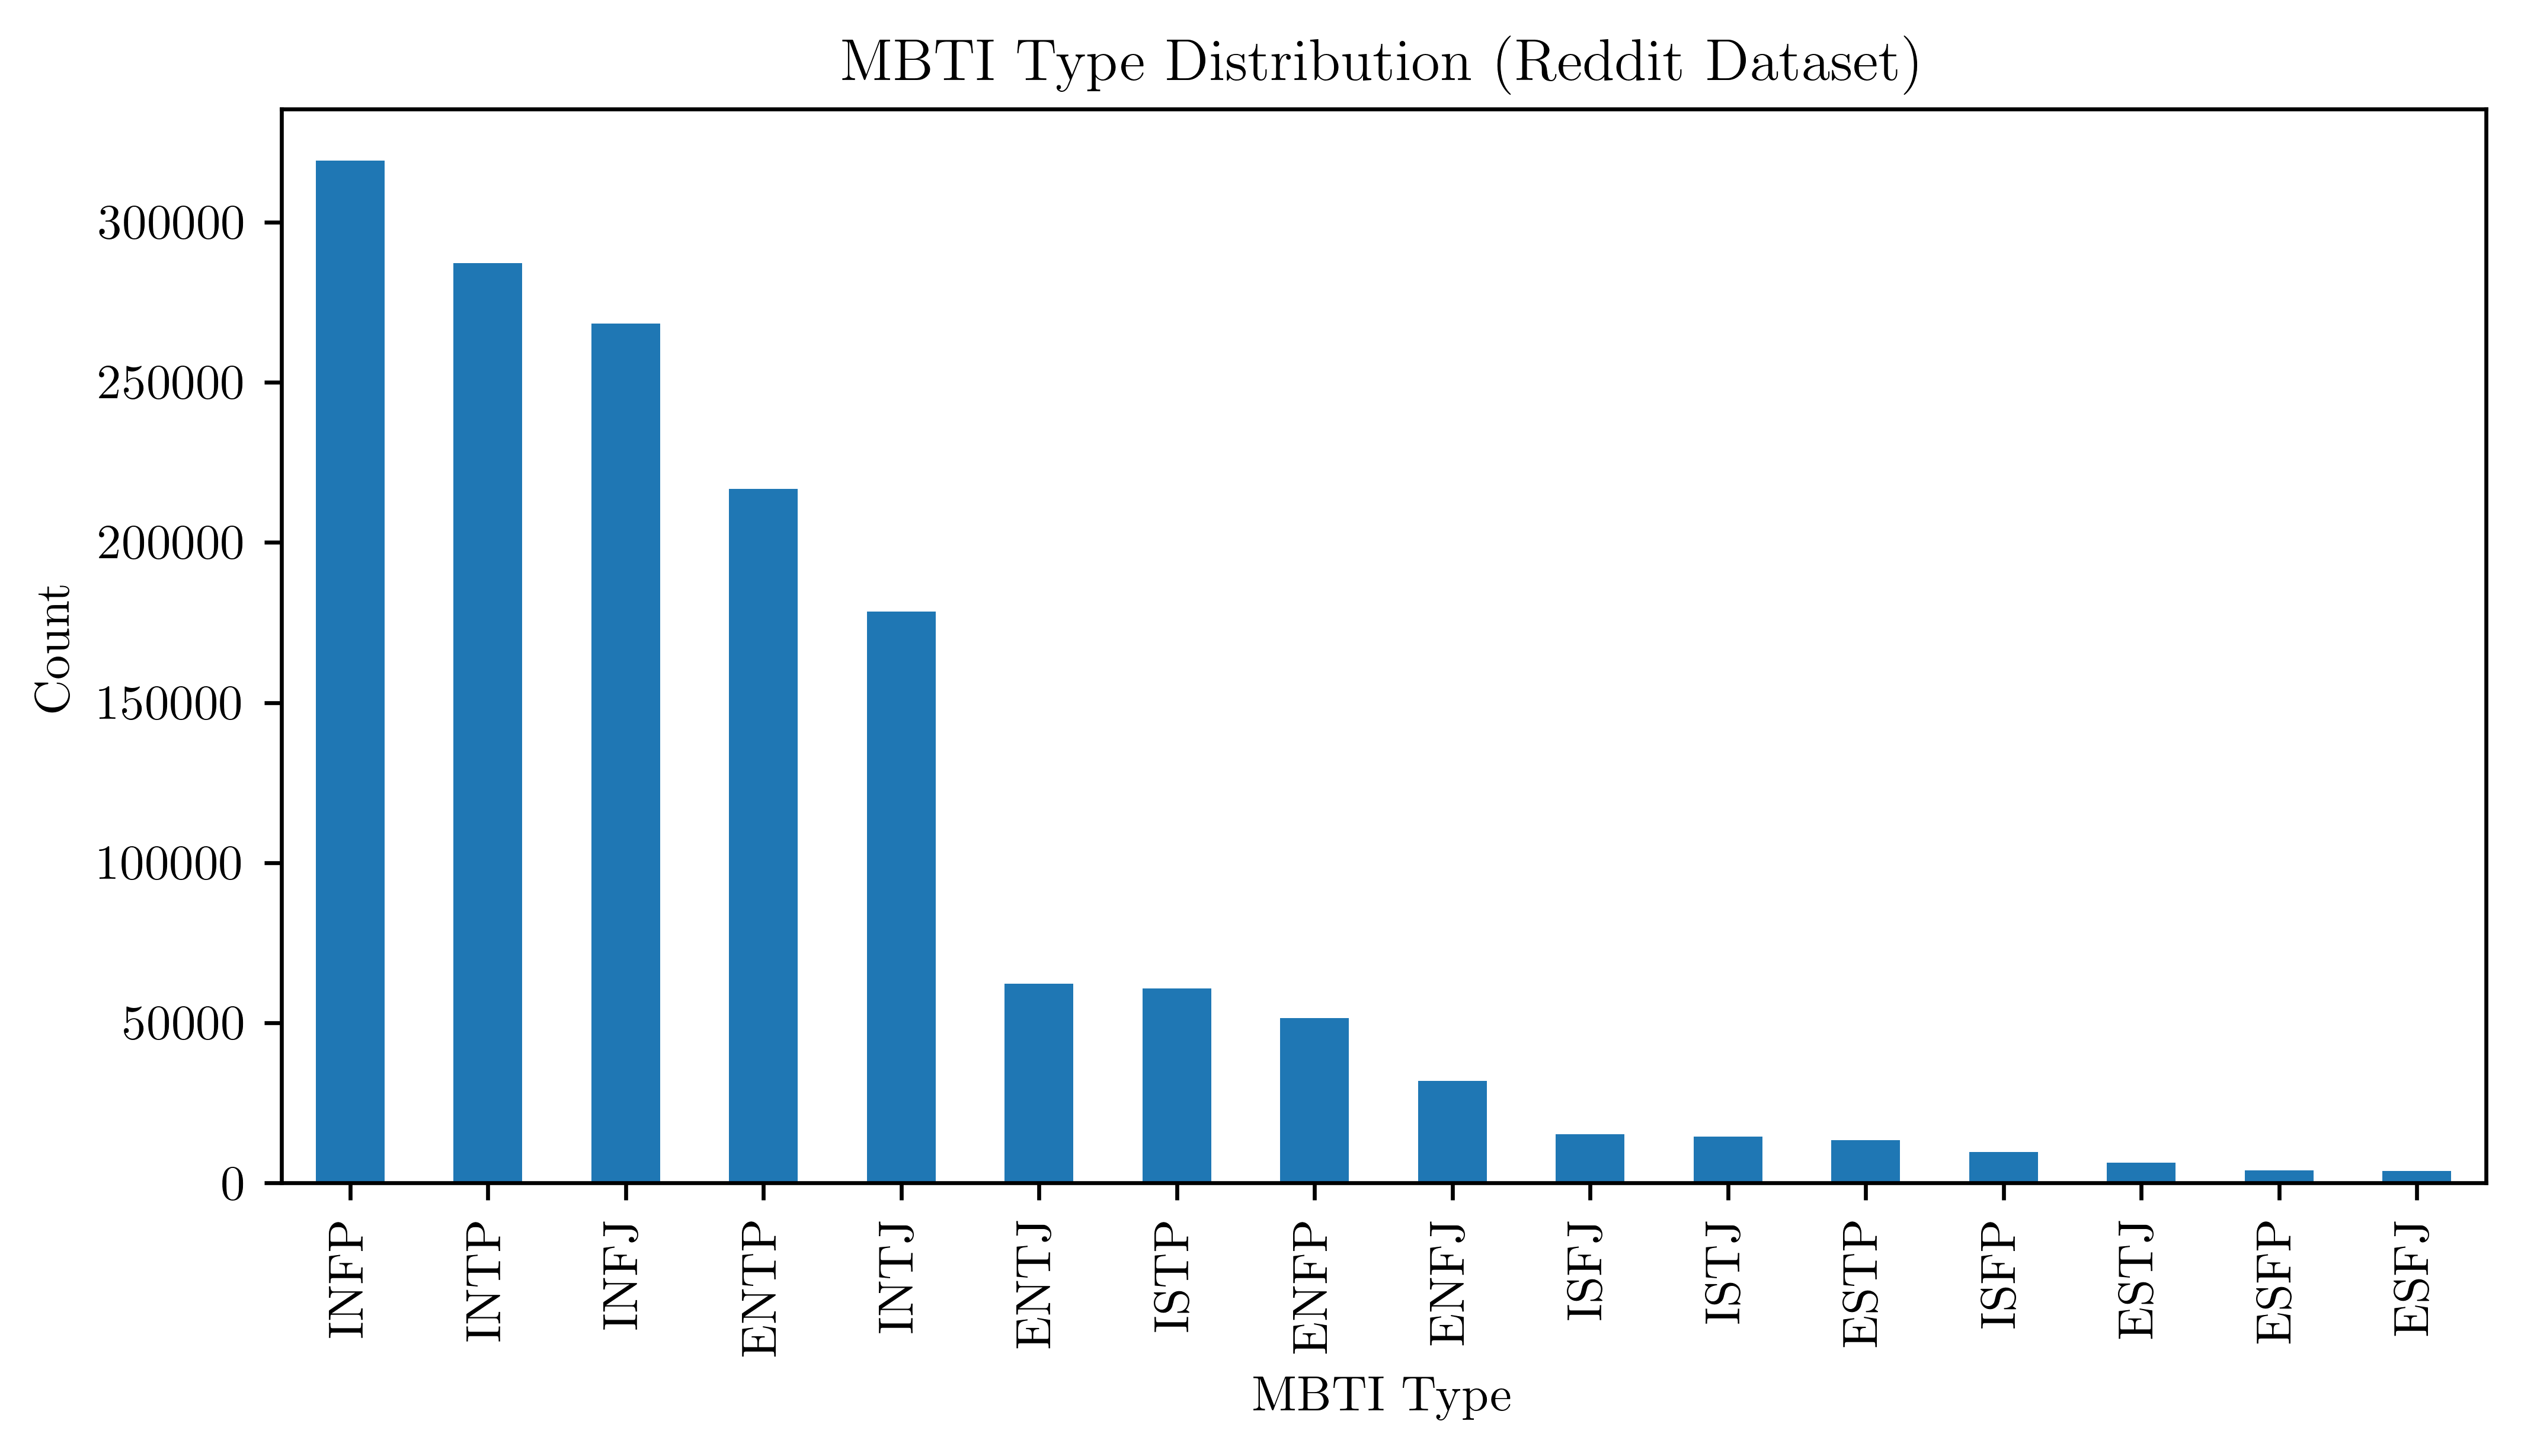
\includegraphics[height=8cm]{../output/visualisations/class_dist_reddit}
		
		\caption{Population distribution of the MBTI types from Reddit}
		
	\end{figure}

		\begin{figure}[h!]
		\centering
		
		\includegraphics[height=9cm]{../output/visualisations/dichotomy_dist}
		
		\caption{Population distribution of the MBTI types when divided into different dichotomies}
		
	\end{figure}

	\begin{figure}[h!]
		\centering
		
		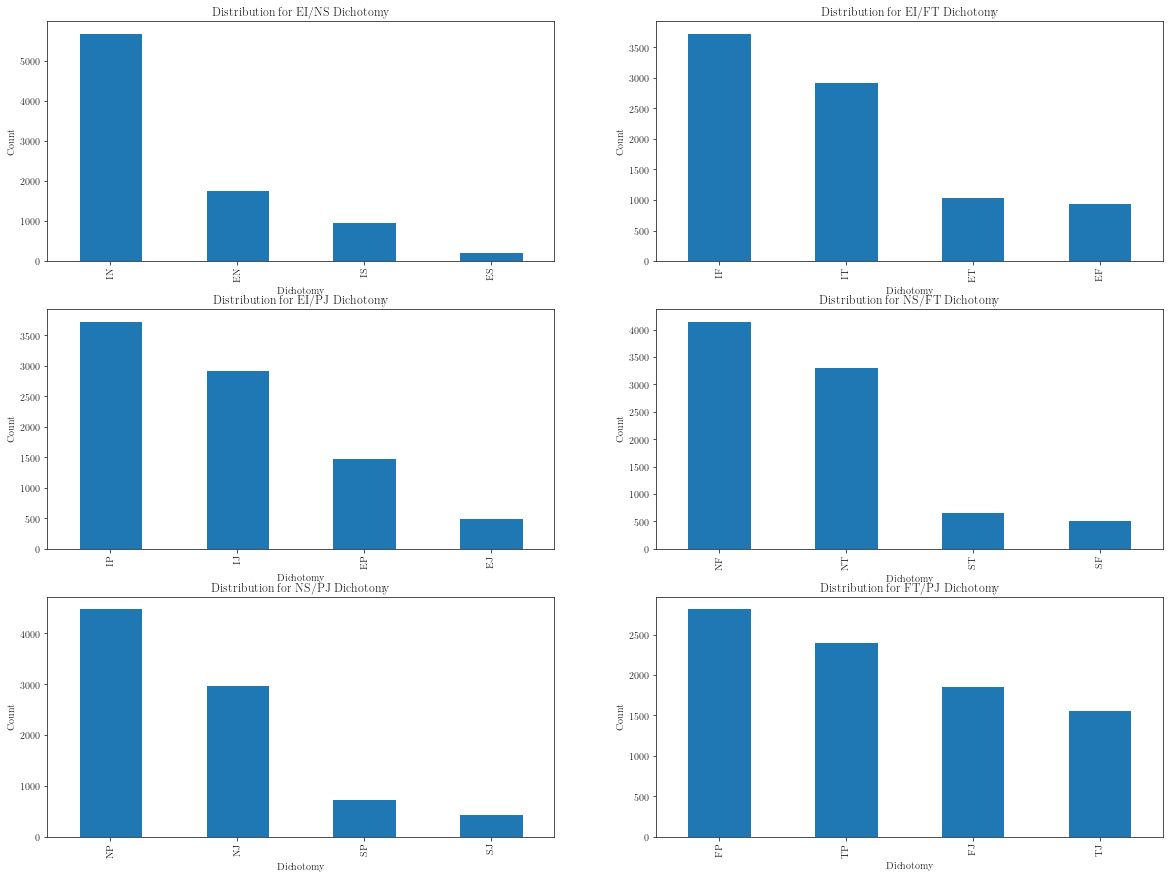
\includegraphics[height=12cm]{../output/visualisations/dichotomy_dist_2}
		
		\caption{Population distribution of the MBTI types when divided into different two-dimentional dichotomies}
		
	\end{figure}

	\begin{figure}[h!]
		\centering
		
		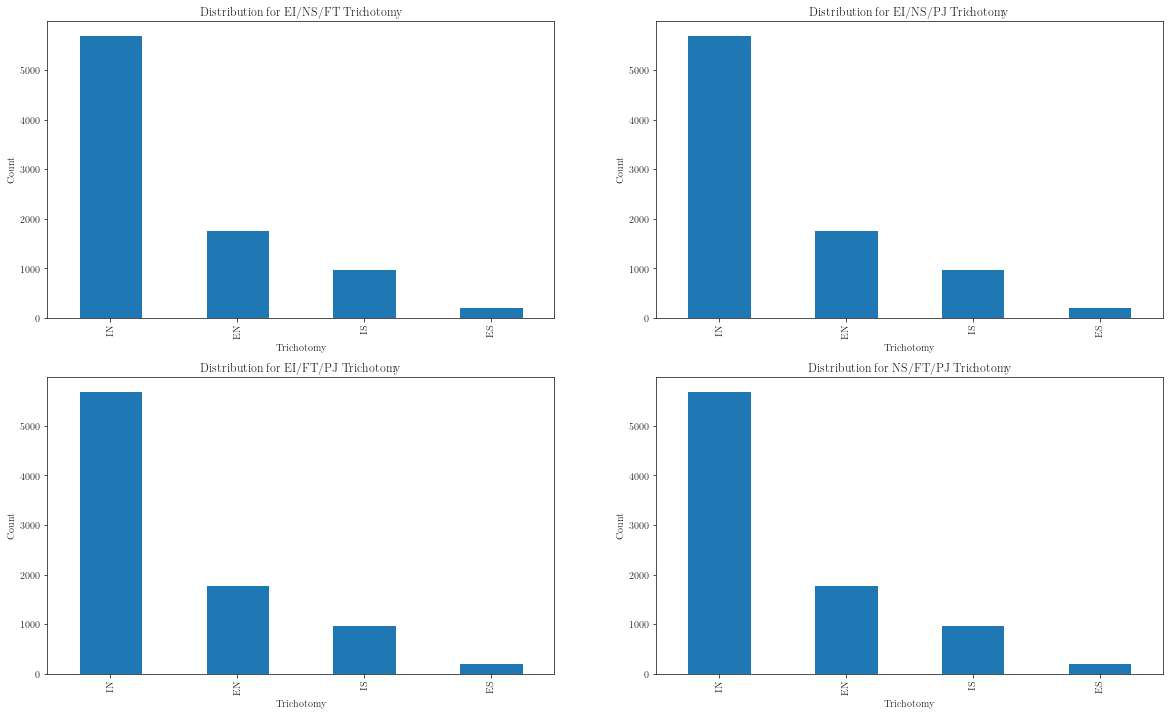
\includegraphics[height=9cm]{../output/visualisations/trichotomy_dist}
		
		\caption{Population distribution of the MBTI types when divided into different trichotomies}
		
	\end{figure}

	\begin{figure}[h!]
		\centering
		
		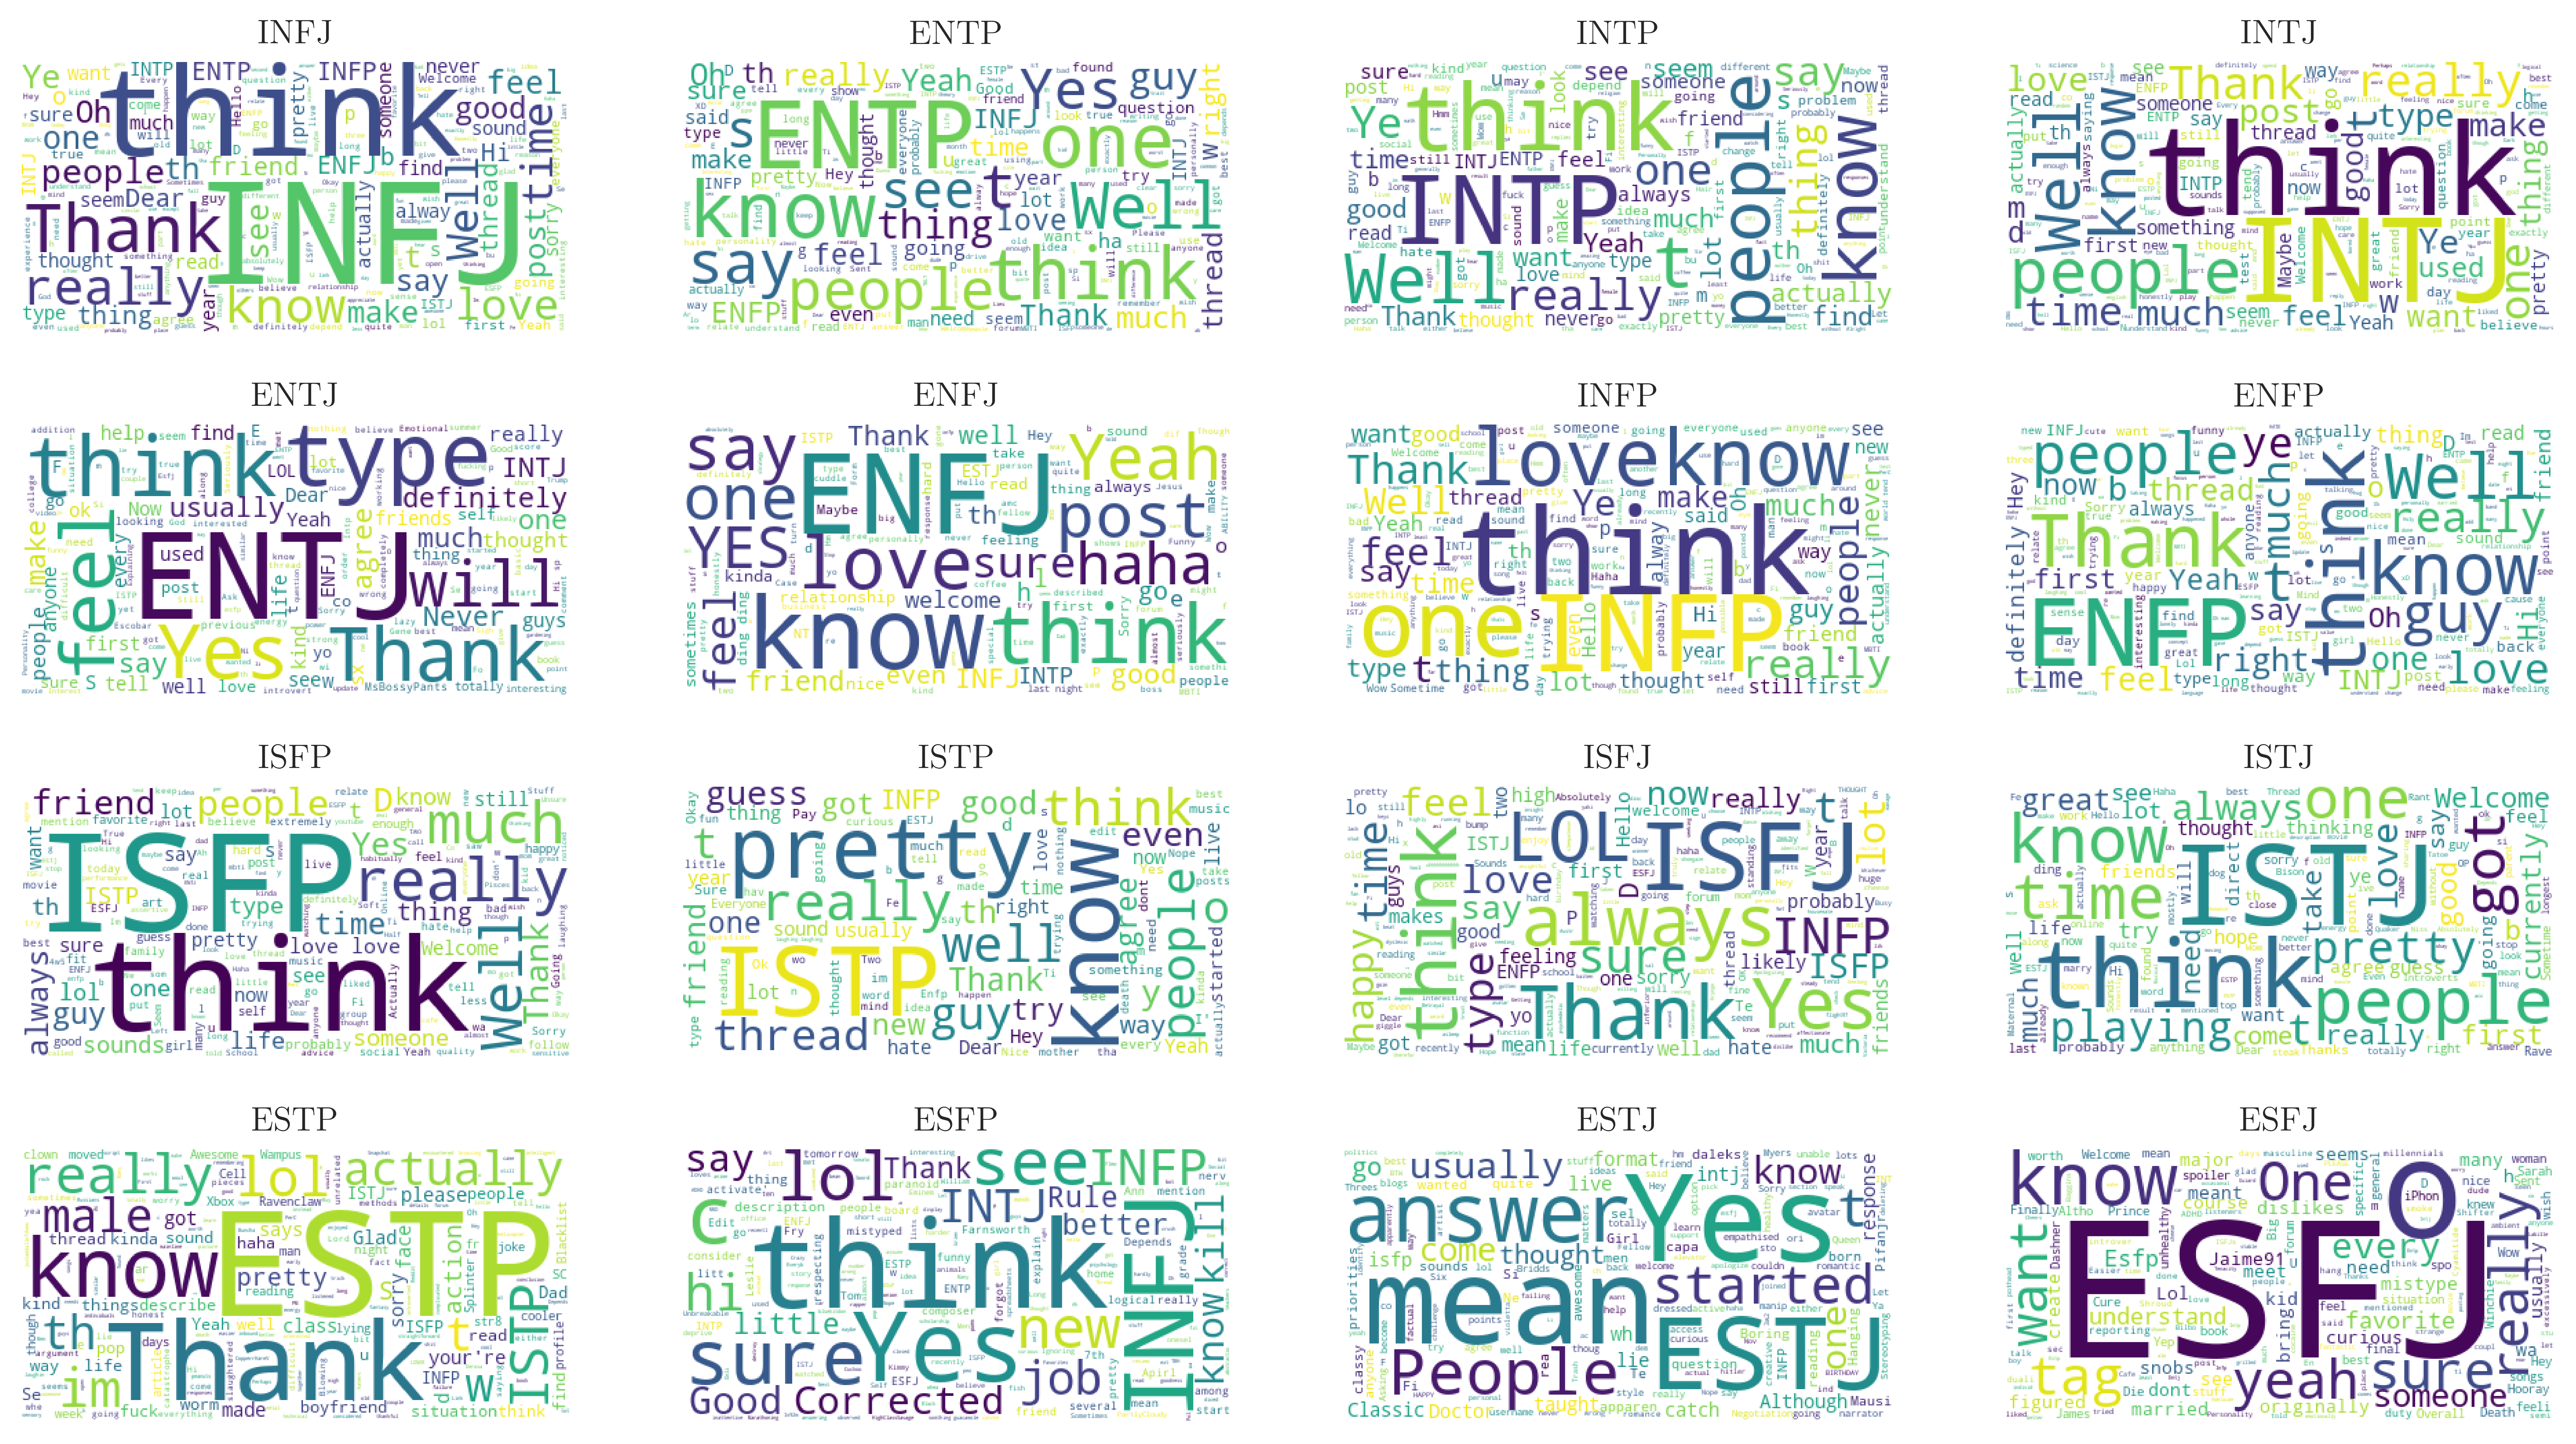
\includegraphics[width=\textwidth]{../output/visualisations/wc}
		
		\caption{Word clouds from each MBTI type}
		
	\end{figure}

	When observing the word clouds in Figure 8, there seems to be an indication that the corpus themselves contain the correct classification. This is to be expected as the data came from a forum based on conversations on personality. Therefore, the removal of these words is one of the considerations that is going to be made when preprocessing the text data. Knowing that the types of words used are different in each class means that there is some confirmation that classification based on text data might be feasible.
	
	\clearpage
	
	\section{Modelling}
	
	On a macro scale, the process of modelling the data will involve the input of the dataset as mentioned above with the objective of obtaining a model that best predicts the MBTI type of the user based on their posts.
	
	\begin{figure}[h!]
		\centering
		
		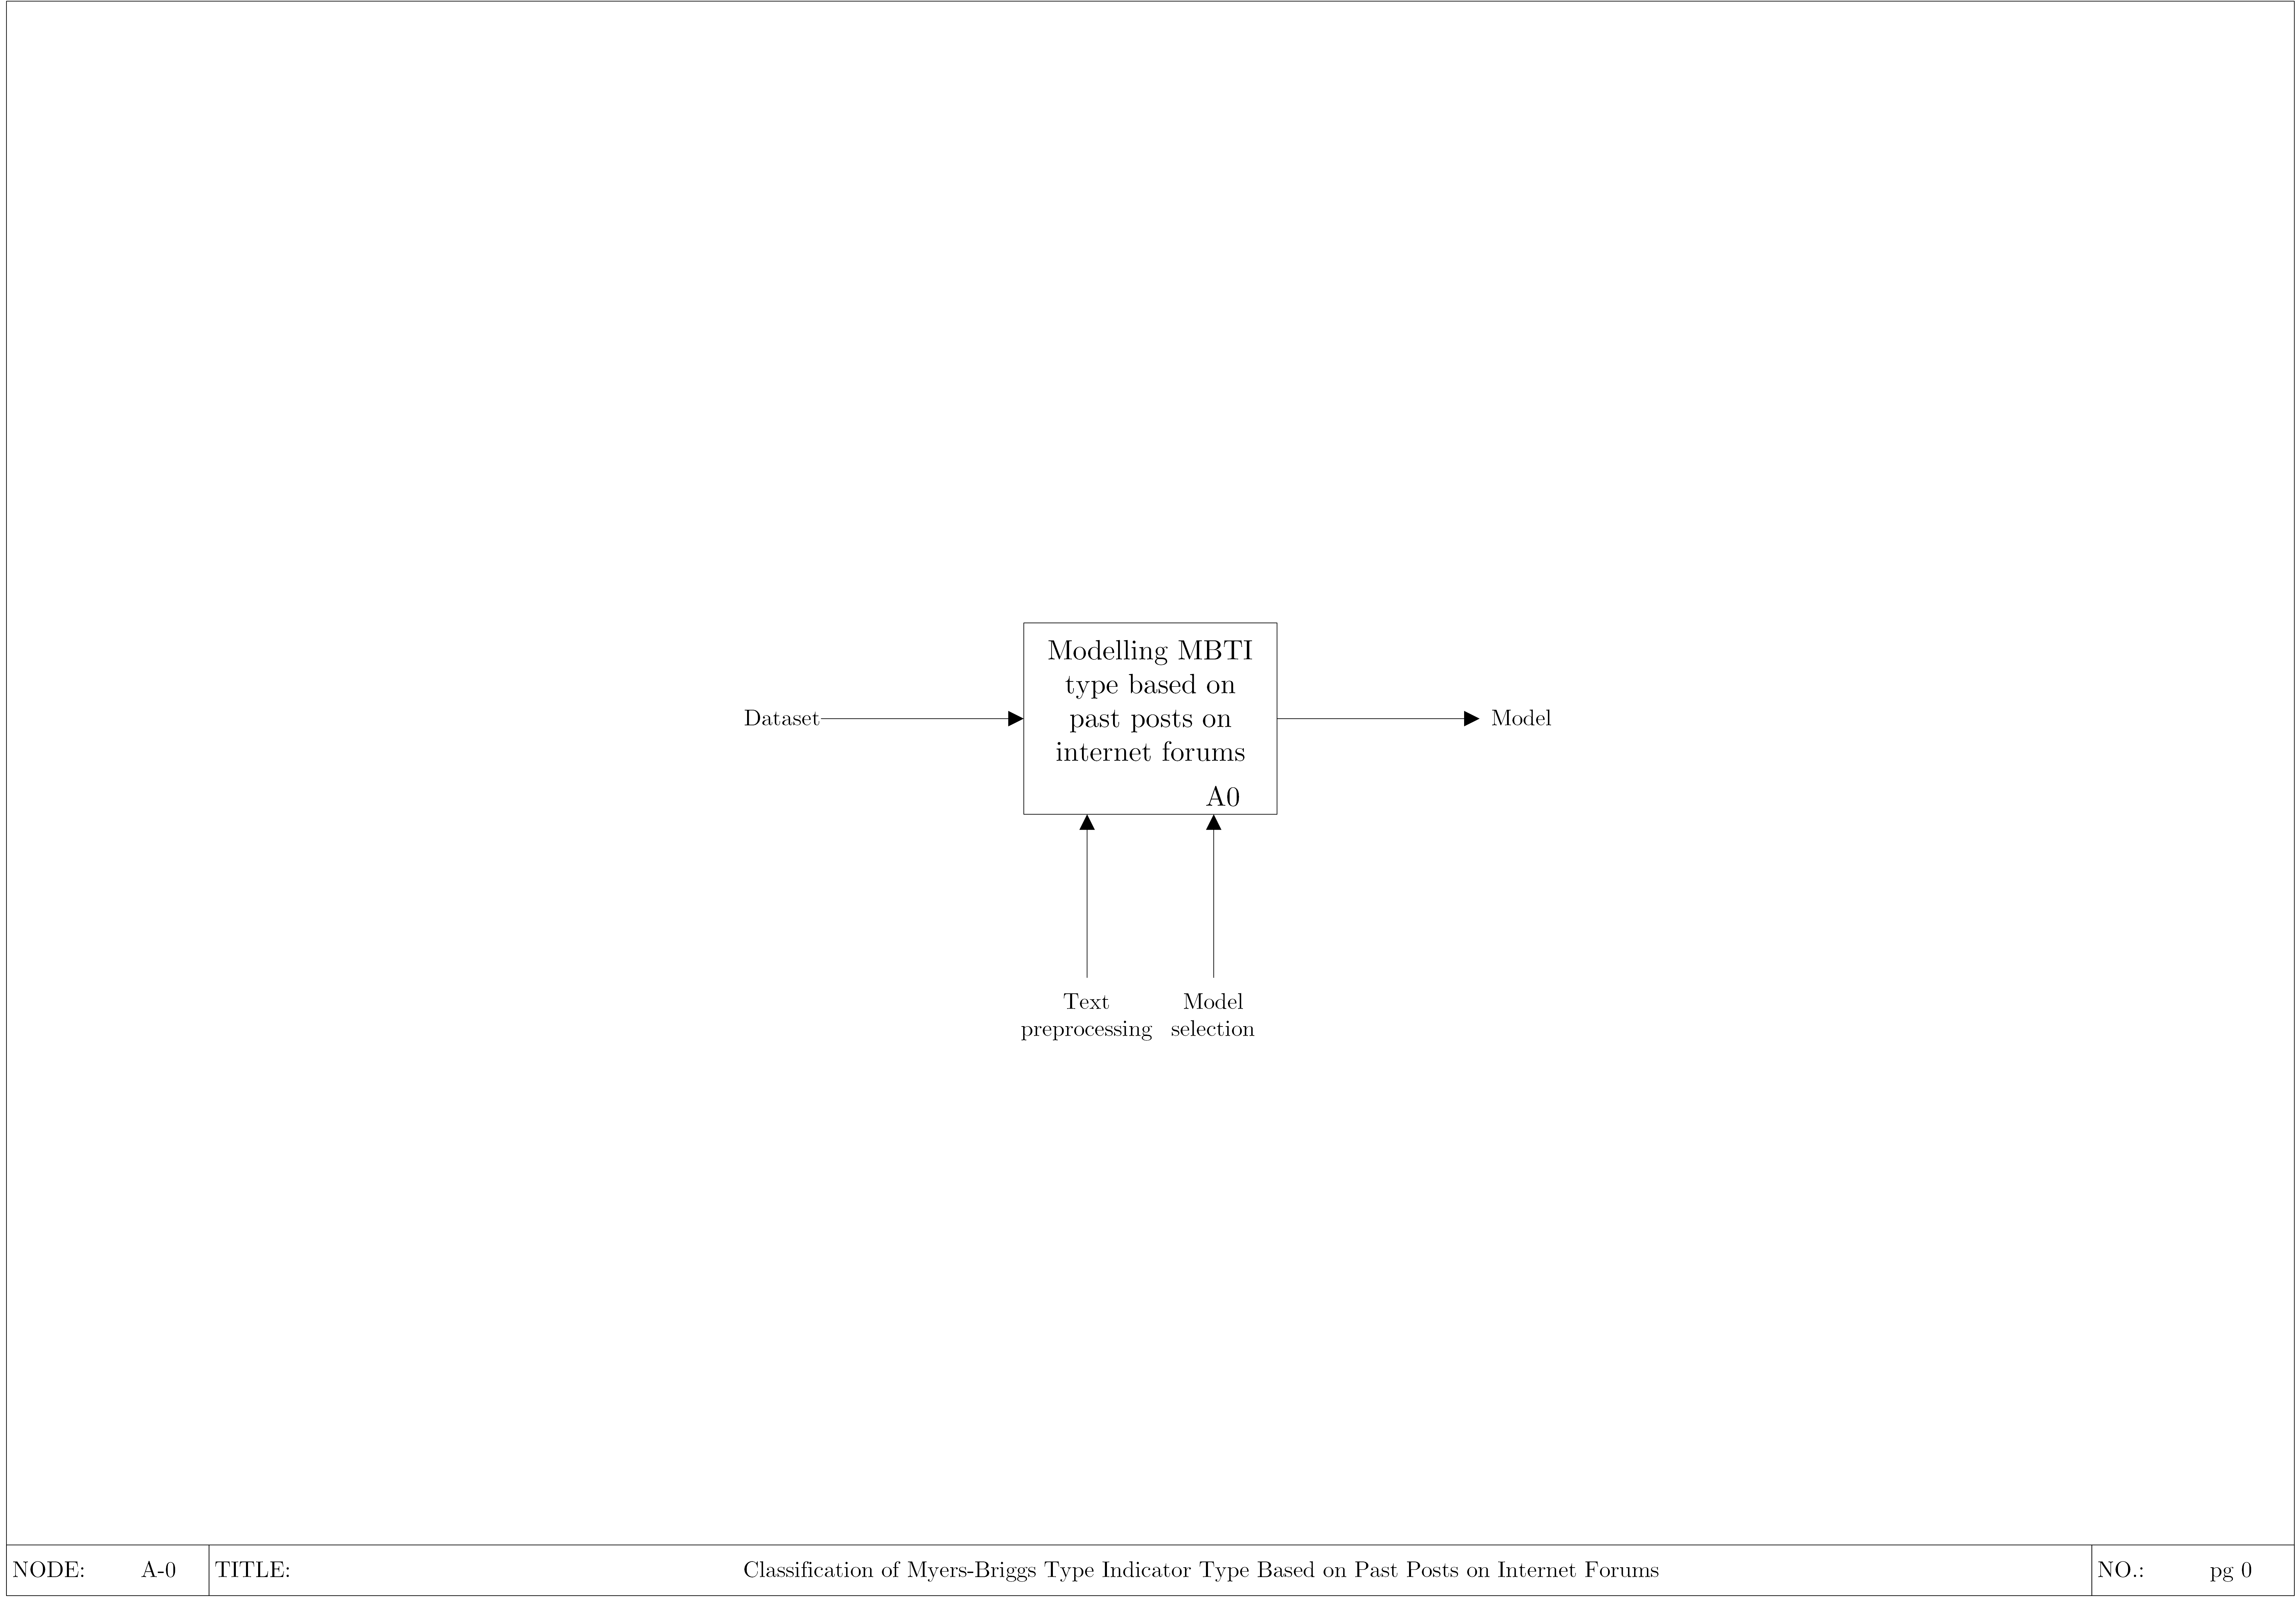
\includegraphics[width=\textwidth]{img/CDS0}
		
		\caption{Macro view of the modelling process}
		
	\end{figure}

	
	\begin{figure}[h!]
		\centering
		
		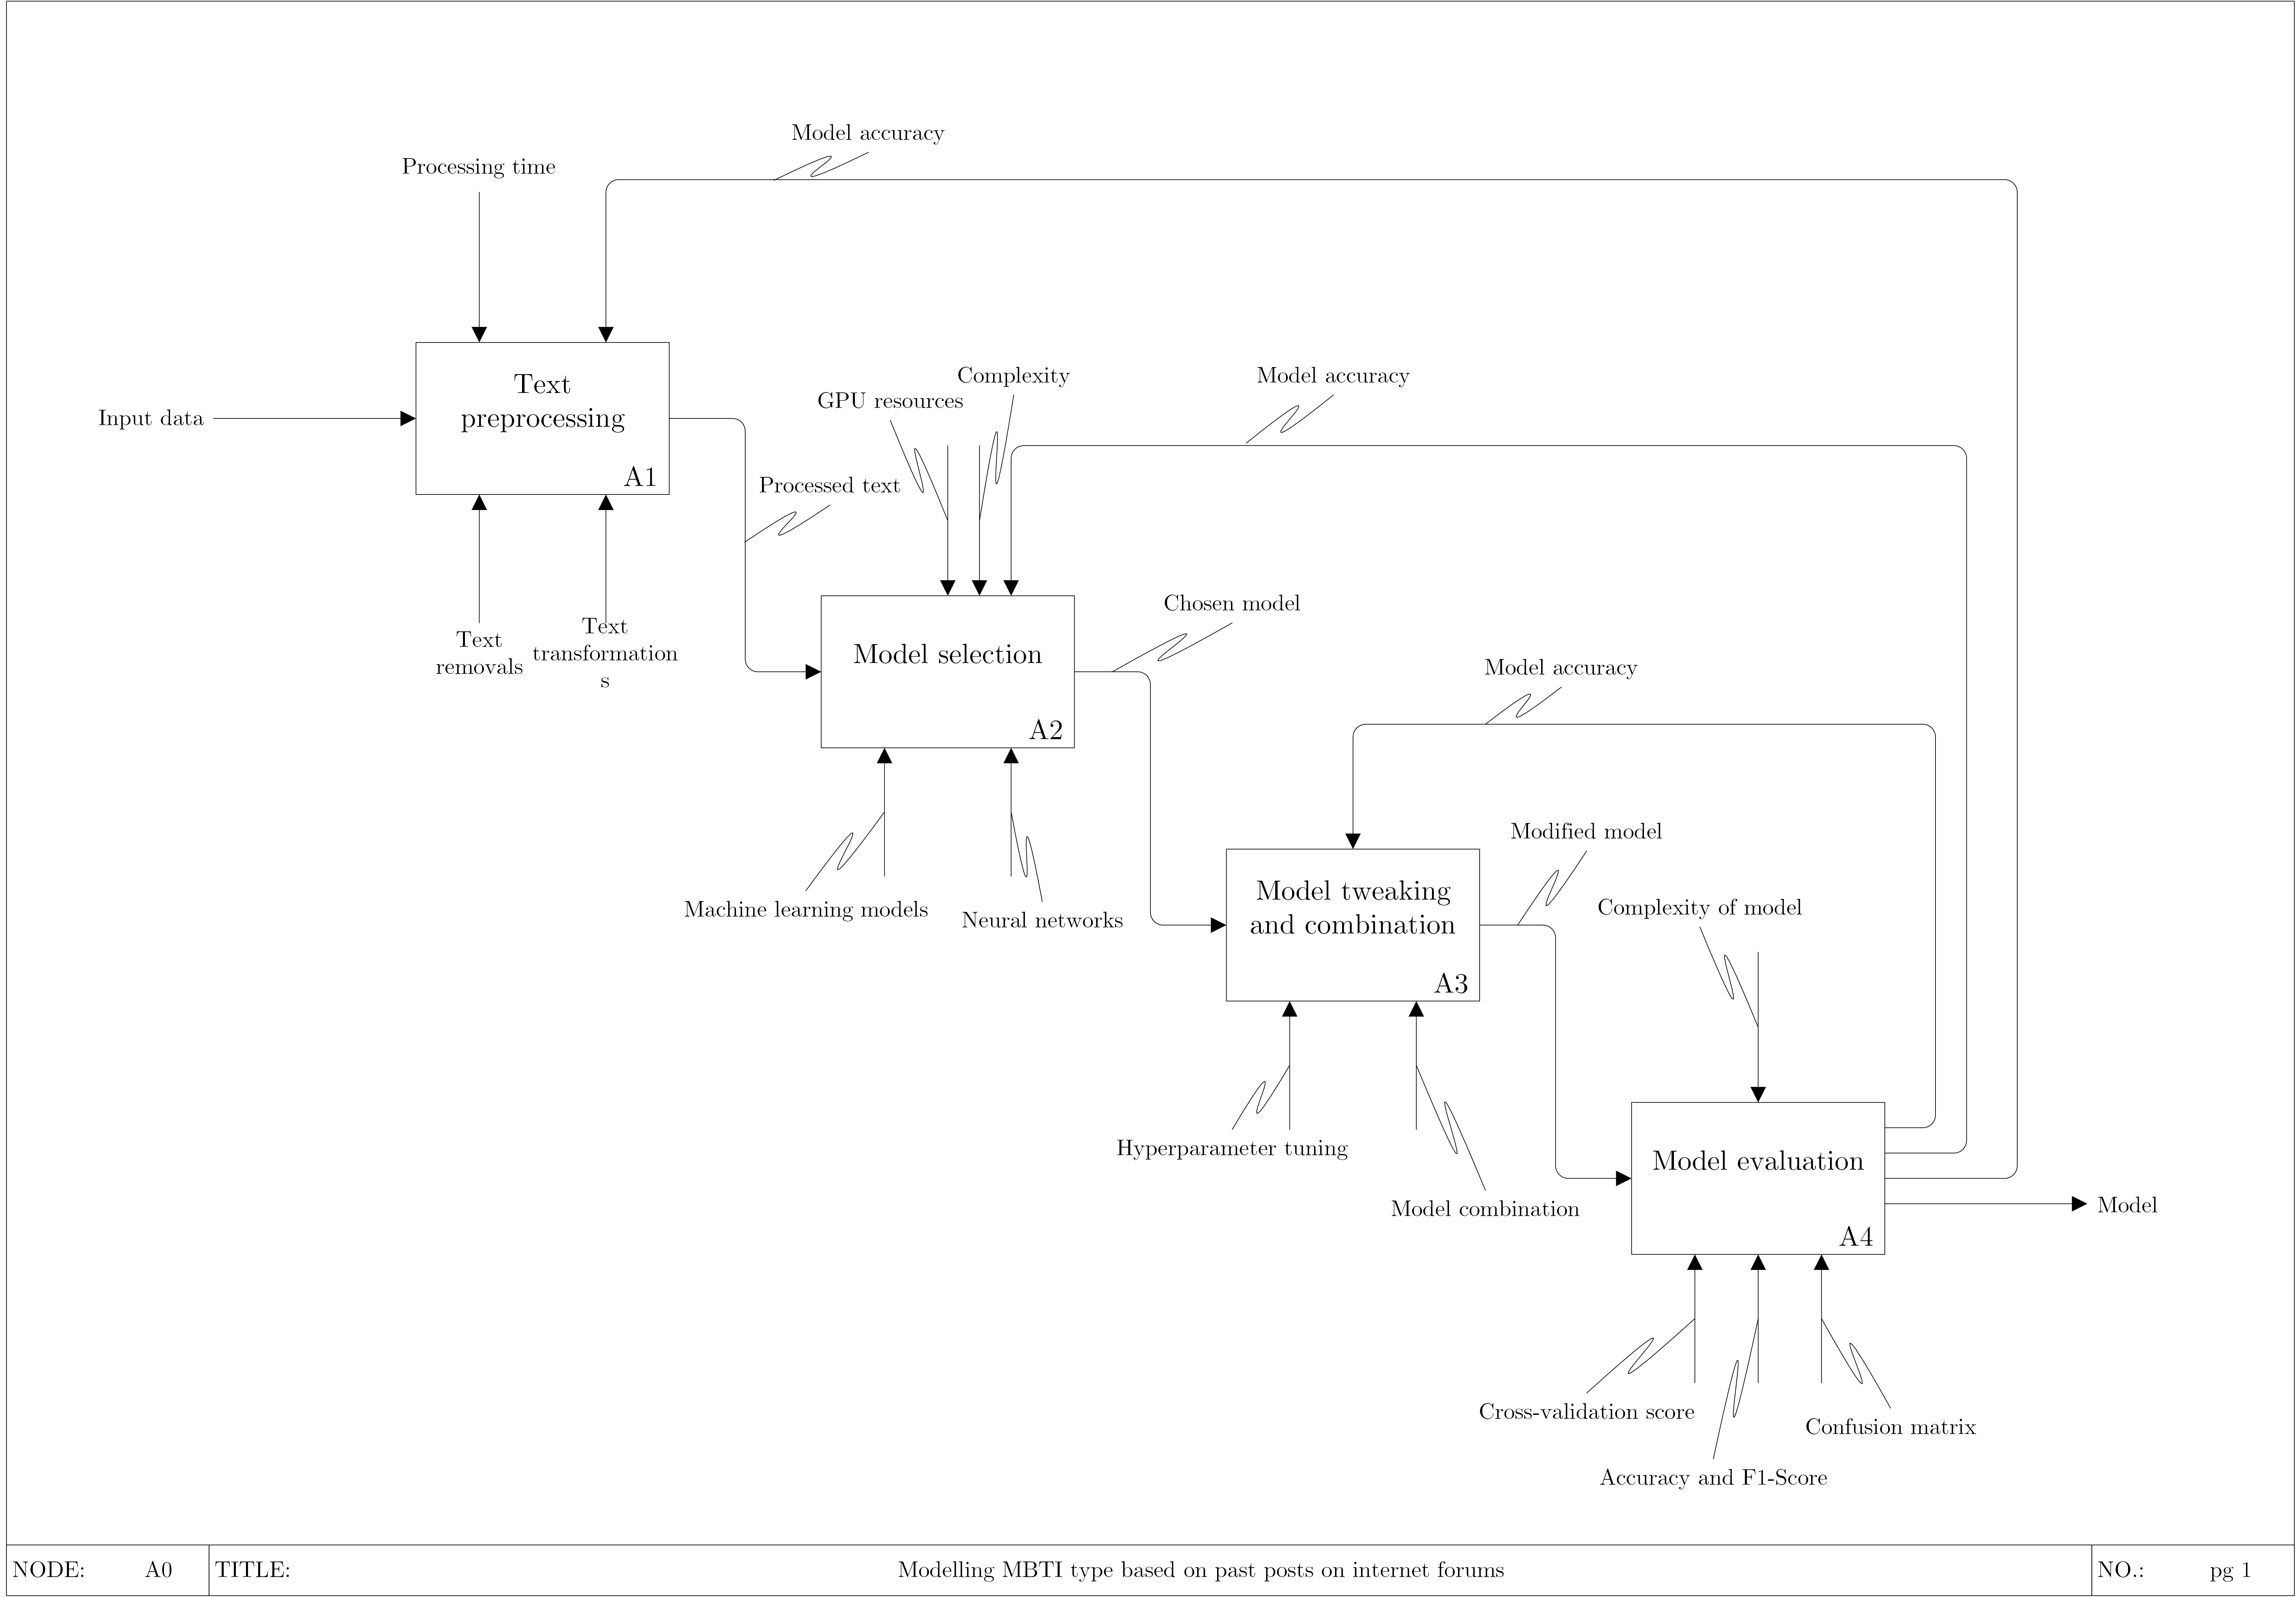
\includegraphics[width=\textwidth]{img/CDS}
		
		\caption{More in-depth view of the modelling process}
		
	\end{figure}
	
	Observing the process a little bit deeper, there are roughly four main steps, happening somewhat sequentially, though there will be many iterations based on the model accuracy. The data goes through text preprocessing first, involving removals of irrelevant data and transformations required for the models being tested. Here, processing time is a concern as it will also impact not only the modelling, but also the prediction time using the model. The processed text is then fed into the model selection process where several candidates from machine learning and neural network models are chosen and tested based on their accuracies. Again, there are constraints based on the resources had and the complexity of the model also affects the time taken in training, knowing the relatively limited timespan had in going through the various models. After the top few models are chosen, they will be tweaked and even be combined together, and the ones with the highest accuracy will be chosen as the final model. The evaluation process will depend on the complexity of the model, potentially including not only accuracy, classification reports, and confusion matrices, but also cross-validation scores. The ROC/AUC curve was also considered, but knowing the unevenness of the MBTI types in the dataset, it was decided that it will not be as reliable as the F1-score.\autocite{MachineLearningF1}
	
	
	\clearpage
	\section{Text preprocessing}
	
	\subsection{Cleaning}
	
	As with any kind of text corpus, the cleaning thereof is required before converting them into vector representations. The main considerations in the model will be as follows:
	
	\begin{enumerate}
		\item Changing all the text into lower case. This is in order to prevent fragmentations of identical words in different cases.
		\item Removal of URL links, mentions, and hashtags. Those sets of words usually do not add to the meaning of the sentence. Sometimes they are accompanied by symbols, which makes the overall message more indistinct.
		\item Expansion of contractions. This is to preserve more meaning and to prevent further fragmentations of words with identical meaning in different forms.
		\item Removal of accented characters. This is, again, to prevent fragmentations (e.g. Naïve vs Naive).
		\item Removal of non-alphabetic characters. The assumption is that numeric and punctuation characters do not add much meaning to the corpus.
		\item Removal of English stop words. This is to reduce the noise associated with common English words that do not specifically point to a meaning.
		\item Lemmatising the words. This is to reduce fragmentations even further by combining words of different nature into the same lemma.
		\item Removal of single characters and extra whitespace. This is to reduce the information noise in the corpus.
	\end{enumerate}

	This will form the baseline for the preprocessing framework. There will be modifications to this during the model tweaking and combination stage. The decision to keep the MBTI type words in the corpus is done as it keeps the context of the dataset intact---that it is the natural conversation topic in a forum centred around the self and personality types.
	
	\subsection{Word embeddings}
	
	There are three different choices that were compiled: GloVe, FastText, and Paragram.\autocites{GloVeGlobalVectors}{EnglishWordVectors}{JohnWieting} These three will be tested during the model tweaking and combination stage. The baseline word embedding chosen will be FastText due to its advantage of being able to work well with rare and unrepresented words.\autocite{GloVeFastTextTwo} Moreover, its vector file is the smallest of the three.
	
	\clearpage
	\section{Model selection}
	
	\subsection{Classical machine learning models}
	
	\subsubsection{Support Vector Machine}
	The model was implemented via GridSearchCV with 3 cross validation folds to facilitate hyperparameter tuning to enhance model performance. Support vector machine was used as it is a powerful classifier which divides data points according to a decision boundary. The highest accuracy score that SVM managed to generate was 0.63.
	\subsubsection{Random Classifier}
	The model was implemented via GridSearchCV with 3 cross validation folds to facilitate hyperparameter tuning to enhance model performance. The dataset is fed into the model and is divided into smaller components and are constructed into decision trees. Afterwards, they are made to predict and the tree with the most number of votes will have its prediction result set as the final random forest’s prediction result. The accuracy result obtained is 0.38.
	\subsubsection{Logistic Regression}
	The model was implemented via GridSearchCV with 3 cross validation folds to facilitate hyperparameter tuning to enhance model performance. The model follows a sigmoid function whereby if the output is more than 0.5 it will result in a y-value of 1 and otherwise 0. The accuracy result recorded is 0.61.
	\subsubsection{Decision Tree}
	The most suitable Attribute Selection Measures will be selected to divide the data and it will be further sectioned off to build trees until the condition of a tree’s child node is met. The accuracy for this model is 0.21.
	\subsubsection{XGBoost Classifier}
	Unlike traditional ML models this classifier was faster than its counterparts but however in terms of performance it was poorer. Even though it was regarded to be superior. It works via an optimised form of gradient boosting algorithms to enhance the overall performance. The accuracy for this model is 0.15.
	\subsubsection{CatBoost Classifier}
	Similar to XGBoost, CatBoost is another gradient boosting algorithm which is designed to lessen overfitting and maintaining a loss rate across training, validation and testing. It is very robust to the point that XGBoost adapts some of its features. The accuracy result of the model is 0.67. Hence, it is very evident that unlike other classical and gradient boosting models the CatBoost algorithm is far superior and high-performing.
	\subsubsection{Gaussian Naive Bayes}
	The accuracy obtained from this model is 0.38.
	\subsubsection{Multinomial Naive Bayes}
	This model specifically caters to discrete variable classification, which would mean entities like word counts. As a result, the usage of token count matrix is apt for this model due to it being compatible with integers rather than fractional values. Hence, the accuracy obtained is relatively higher than the most of the models with a value of 0.58.
	\subsubsection{Complement Naive Bayes}
	This model serves to improvise on the shortcomings of the previous model by eliminating prior assumptions and aiding dataset which are very disproportionate across the classes. The accuracy obtained is 0.63.
	\subsubsection{Categorical Naive Bayes}
	This models performs well for discrete features which are categorical distributed, similar to Multinomial Naive Bayes. The accuracy scored for this model was relatively higher with a value of 0.63 again.
	
	
	\subsection{Neural Networks}
	
	Both the neural network models below are used with the Adam optimiser with the Cross Entropy Loss function, and the MBTI types are encoded into integers using the LabelEncoder function from Scikit-learn.
	
	\subsubsection{Long-Short Term Memory (LSTM)}
	
	By building a model with an LSTM single direction layer with hidden dimension size of 256 and a SimpleAttention layer, the accuracy of about 0.64 is attained in the validation set. To implement self attention, there are several dimensional changes have been done. Apart from that, LogSoftmax was used in the end of the forward function to convert a vector of numbers into a vector of probabilities. 
	
	\subsubsection{Convolutional Neural Network (CNN)}
	
	At first, the two-dimentional CNN layer with five filters did not work as well, giving an accuracy of around 0.67. However, when the text preprocessing was modified to exclude the removal of single characters, lemmatisation, and the removal of stop words, the accuracy jumped to around 0.68. This is a first indication that these processes can be detrimental to the model's performance.
	
	\subsection{Conclusion}
	
	While CatBoost seemed to be very promising, the ultimate choice here is to attempt to use a CNN model due to its greater flexibility. Also, LSTM will also be considered as an extension to the CNN model with the hopes of improving the accuracy. Therefore, the baseline model used to tweak and combine will be the CNN model that excluded the removal of single characters, lemmatisation, and the removal of stop words.
	
	
	\newpage
	\section{Model tweaking and combination}
	
	There were a few comparisons made in order to find out ways to improve the model further.
	
	\subsection{Text preprocessing}
	
	As outlined earlier, the accuracy seemed to be better when the single characters and stop words are not removed and the words are not lemmatised. However, there is also the question of which word embedding model to use. When using GloVe, the accuracy reached 0.70, while using Paragram yielded 0.71. Therefore, the usage of Paragram seems to be better.
	
	Knowing that the model will perform poorly on the whole sixteen classes, it is then decided that the final models will only cover the top six classes such that it can be a more reliable model.
	
	\subsection{Tweaks and combinations}
	
	Using the baseline CNN model with FastText, the tweaks included the changing of dropout rates and the number of filters. However, this did not improve the accuracy much. Therefore, an LSTM layer is inserted after the convolutional layer in the hopes of improving the accuracy. With that, the accuracy went up to around 0.78. However, even though the Paragram word embedding seemed better in the CNN-only model, when using it with this new model, the accuracy was worse at around 0.71.
	
	\subsection{Conclusion}
	
	Therefore, the best model in this case is the CNN-LSTM model with the FastText word embedding. The preprocessing of the text does not include the removal of single characters, lemmatisation, and the removal of stop words, which improves the time taken to both model and predict significantly.
	
	\begin{figure}[h!]
		\centering
		
		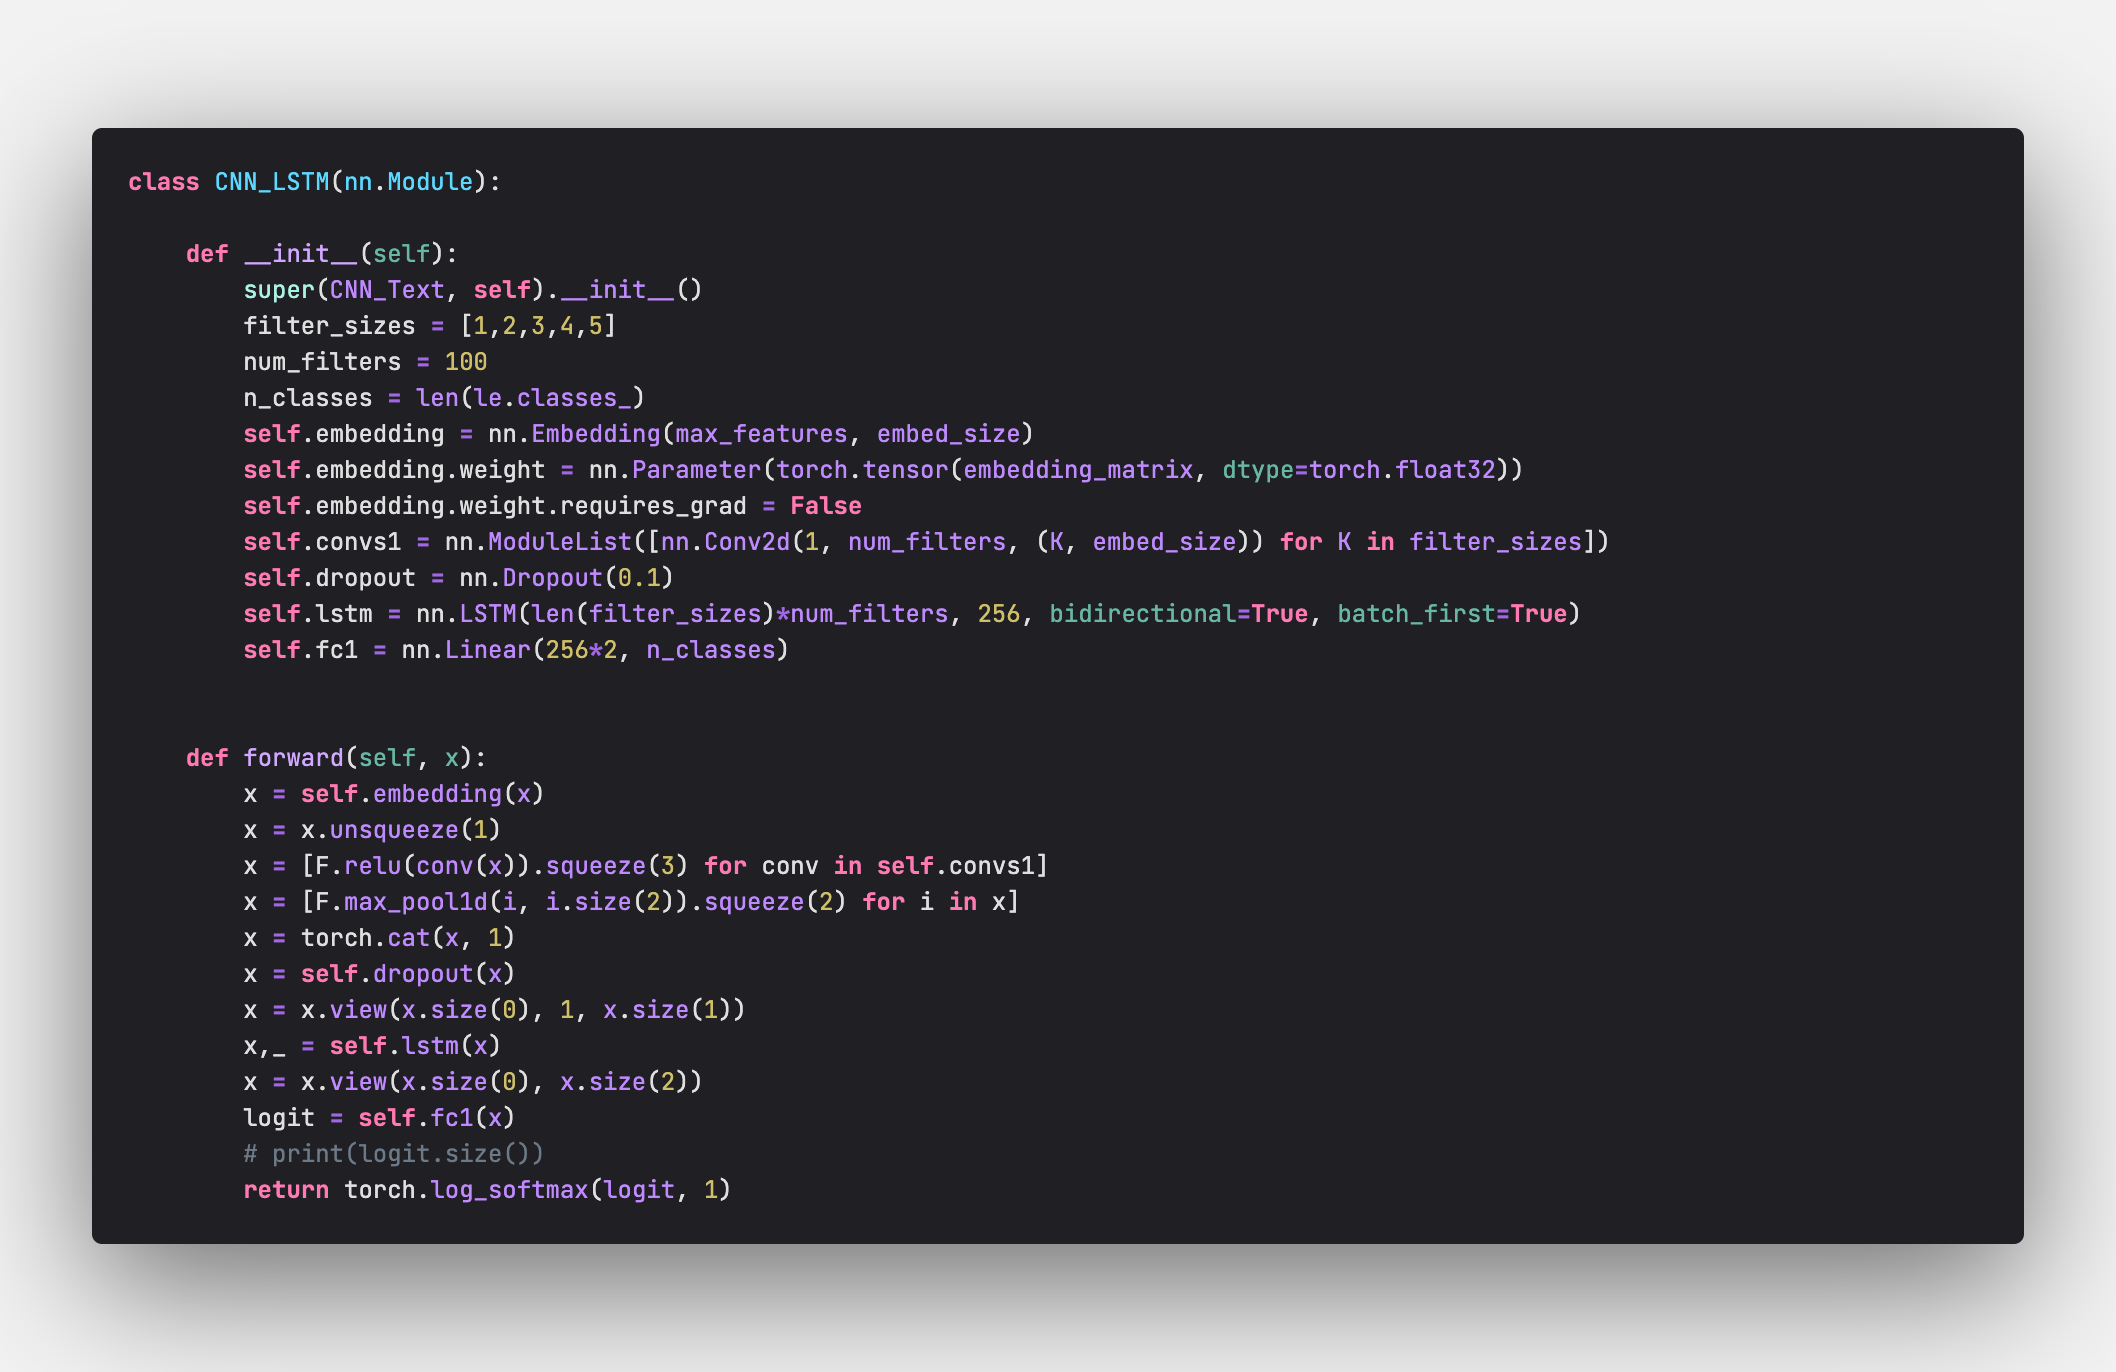
\includegraphics[height=9cm]{../output/visualisations/code}
		
		\caption{Code for the model chosen}
		
	\end{figure}
	
	\newpage
	
	\section{Model evaluation}
	
	Due to the model chosen being a neural network, it was decided that a cross-validation technique will be impractical. As such, the evaluation will be in the form of a confusion matrix and classification report.
	
	\begin{table}[h!]
		\centering
		\begin{tabular}{l|llll}
			& Precision & Recall & F1-Score & Support \\ \hline
			ENFP         & 0.77      & 0.75   & 0.76     & 169     \\
			ENTP         & 0.70      & 0.71   & 0.71     & 171     \\
			INFJ         & 0.81      & 0.76   & 0.78     & 368     \\
			INFP         & 0.78      & 0.84   & 0.81     & 458     \\
			INTJ         & 0.82      & 0.75   & 0.79     & 273     \\
			INTP         & 0.78      & 0.80   & 0.79     & 326     \\
			Accuracy     &           &        & 0.78     & 1765    \\
			Macro Avg    & 0.78      & 0.77   & 0.77     & 1765    \\
			Weighted Avg & 0.78      & 0.78   & 0.78     & 1765   
		\end{tabular}
		\caption{Classification report for the model}
		\label{tab:my-table}
	\end{table}
	
	\begin{figure}[h!]
		\centering
		
		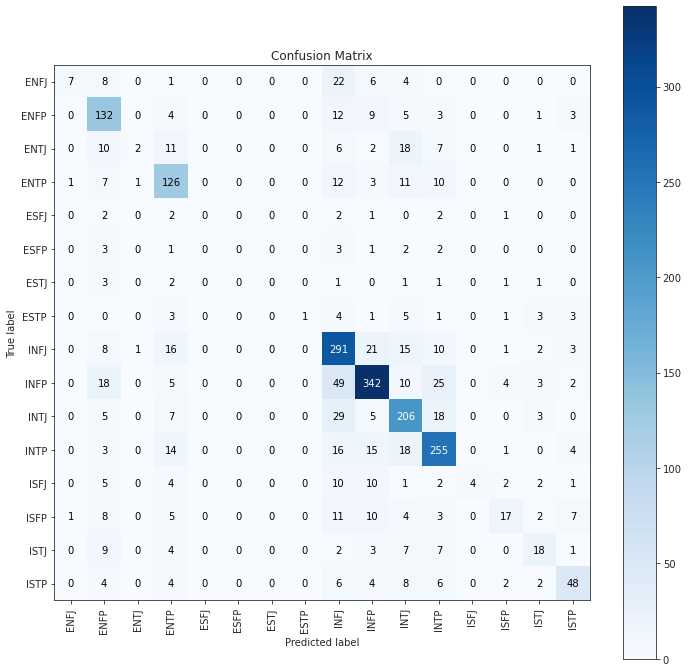
\includegraphics[height=11cm]{../output/visualisations/confusion}
		
		\caption{Confusion matrix of the model's prediction on the validation set}
		
	\end{figure}
	
	From the classification report and the confusion matrix, it can be concluded that the model works relatively well for the majority data, but falls short when considering the minority data. Some of the confusions shown are from MBTI types that differ only by one letter, particularly within the J/P dichotomy.\autocite{choongPredictingJudgingperceivingMyersBriggs2021} Other works have shown that this particular dichotomy is quite challenging to predict.
	
	\newpage
	\section{Conclusion}
	
	In conclusion, it seems like it will be very difficult to push the accuracy beyond 0.80. This makes sense when considering the nature and weakness of the MBTI. As this is the aggregation of the past fifty posts by users in a forum, it stands to reason that, knowing that people's MBTI types tend to change over a period of time, the MBTI of a user can change slightly over the course of the fifty posts, affecting the aggregated data. Moreover, the inability for the model to predict the minority data well can be attributed to the lack of data. As such, an improvement to this model will include this in mind.
	
	Another future improvement that can be considered is in exploring the usage of CatBoost a bit further. This is as it has shown a remarkable accuracy. Also, the usage of transfer learning on transformer models such as BERT, ULMFiT, and the likes, can allow for an increase in the accuracy.
	
	In the end, the model is unlikely to have the potential to be generalised to a more public dataset. This is due to the conversation that revolves around the forum being more focused and niche, thus potentially creating bias in the model when exposed to datasets from other sources.\autocite{choongPredictingJudgingperceivingMyersBriggs2021} The issue of uneven numbers in the distribution of the MBTI types is also one challenge in need of solving. Thus, a larger, more even labelled dataset is needed to improve the model.
	
	\newpage
	\printbibliography

\end{document}